\chapter{Diseño}

%%%%%%%%%%%%%%%%%%%%%%%%%%%%%%%%%%%%%%%%%%%%%%%%%%%%%%%%%%%%%%%%%%%%%%%%%%%%%%%%%%%%%%
%%%%%%%%%%%%%%%%%%%%%%%%%%%%%%%%%%%%%%%%%%%%%%%%%%%%%%%%%%%%%%%%%%%%%%%%%%%%%%%%%%%%%%
%DISEÑO DE LA INTERFAZ
%%%%%%%%%%%%%%%%%%%%%%%%%%%%%%%%%%%%%%%%%%%%%%%%%%%%%%%%%%%%%%%%%%%%%%%%%%%%%%%%%%%%%%
%%%%%%%%%%%%%%%%%%%%%%%%%%%%%%%%%%%%%%%%%%%%%%%%%%%%%%%%%%%%%%%%%%%%%%%%%%%%%%%%%%%%%%

\section{Diseño de la interfaz}
El diseño de la interfaz de usuario crea un medio eficaz de comunicación entre los seres humanos y la computadora.


\subsection{Principios de diseño de la experiencia de usuario}
Para poder realizar un diseño de interfaz centrado en el usuario, primero hemos de conocer quiénes y cómo son nuestros usuarios. Durante el desarrollo del modelo de negocio pudimos entrevistar a nuestros posibles clientes (futuros usuarios) y pudimos hacernos una idea de cuál es nuestro nicho de mercado.


En nuestra plataforma, tenemos dos tipos de perfiles: Los pacientes\ref{perf_pac} y los psicólogos\ref{perf_psic}.


\begin{table}[htpb]
\centering
\begin{tabularx}{\textwidth}{|X|X|}
\hline
\rowcolor[gray]{0.9}\multicolumn{2}{|c|}{\textbf{Pacientes}}                                                                                                                                                                               \\ \hline
\textbf{Demografía}                                & España                                                                                                                                                            \\ \hline
\textbf{Edad}                                      & Mayores de 16 años                                                                                                                                                \\ \hline
\textbf{Experiencia laboral}                       & Estudios mínimos                                                                                                                                                  \\ \hline
\textbf{Contexto profesional}                      & Cualquiera                                                                                                                                                        \\ \hline
\multirow{2}{*}{\textbf{Necesidades e intereses}}  & Buscar al psicólogo más adecuado para tratar su problemática.                                                                                                     \\ \cline{2-2} 
                                                   & Reducir las preocupaciones de aquellas poblaciones que no puedan acudir físicamente a una consulta por motivos de desplazamiento, urgencias, estigmas sociales... \\ \hline
\textbf{¿Cuándo y dónde utilizaran este servicio?} & Cuando surja la necesidad de contactar con un psicólogo y a través de un ordenador.                                                                               \\ \hline
\end{tabularx}
\caption{Perfil paciente}
\label{perf_pac}
\end{table}


\begin{table}[htpb]
\centering
\begin{tabularx}{\textwidth}{|X|X|}
\hline
\rowcolor[gray]{0.9}\multicolumn{2}{|c|}{\textbf{Psicólogos}}                                                                                                                                 \\ \hline
\textbf{Demografía}                                & España                                                                                                               \\ \hline
\textbf{Edad}                                      & Mayoría de edad                                                                                                      \\ \hline
\textbf{Experiencia laboral}                       & Estudios superiores                                                                                                  \\ \hline
\textbf{Contexto profesional}                      & Psicólogos con especialidad clínica o sanitaria que estén colegiados para el ejercicio de la actividad profesional. \\ \hline
\textbf{Necesidades e intereses}                   & Conseguir un flujo constante de pacientes.                                                                           \\ \hline
\textbf{¿Cuándo y dónde utilizaran este servicio?} & Periódicamente y a través de un ordenador.                                                                           \\ \hline
\end{tabularx}
\caption{Perfil psicólogo}
\label{perf_psic}
\end{table}


Hacer un diseño centrado en el usuario implica tenerlo presente a lo largo de todo el proceso de diseño y tratar de entender cuáles son sus necesidades, intereses y limitaciones.


\subsection{Principios de diseño de la interfaz de usuario}

\subsubsection{\textit{Layout}}
Nuestra interfaz seguirá la regla de los tercios para ayudar a concretar el enfoque del usuario. La regla de los tercios es una forma de composición para ordenar objetos dentro de la imagen al dividirla en nueve partes iguales utilizando dos líneas imaginarias paralelas y equiespaciadas de forma horizontal y otras dos con la mismas características de forma vertical. Los puntos donde se cortan las líneas son los puntos de intersección y sirven para distribuir los elementos de la página. Entre los puntos de intersección se ha de ubicar el centro de atención para crear una imagen estéticamente agradable y equilibrada\cite{georgefield1845}.


La librería Bootstrap, que es una de las librerías escogidas para el diseño de la página, posee un sistema de cuadrículas\cite{bootstrap_grid_basic} que permite dividir la página en filas y columnas. La cuadrícula siempre divide la página en 12 columnas. Como 12 es múltiplo 3, se puede aplicar fácilmente la regla de los tercios a este sistema de cuadrículas.


Por otra parte, también se debe tener en cuenta el público que va a tener nuestra página a la hora de disponer los objetos en ella. La jerarquía visual es importante porque dirige la atención de los ojos del usuario. En nuestro caso, nuestra población es occidental, por lo que el usuario comienza a leer la página desde la esquina superior izquierda. Por este motivo, es interesante situar el logo de nuestra plataforma en esta esquina y la navegación a su lado de forma horizontal.


\subsubsection{Colores}
En la página predominan los colores que, para nuestros futuros usuarios pertenecientes a la población occidental, transmiten:


\begin{itemize}
\item Verde: Seguridad, salud
\item Azul: Seguridad, confianza, estabilidad, veracidad, lealtad
\end{itemize}


El verde y azul son colores análogos, puesto que se encuentran uno pegado a otro en la rueda de color.


Es importante tener en cuenta la cultura de nuestros usuarios, puesto que entre culturas   pueden existir connotaciones de los colores totalmente opuestas.


Para el color de las letras se han utilizado el blanco y el negro (colores neutros) y hacen contraste con el color predominante del background y de los elementos de la página.


\subsection{Fuentes y tipografía}
La tipografía predominante en toda la página es Lato\cite{lato}, pero para aquellos mensajes que queramos resaltar en algún momento puntual se utilizará Merriweather\cite{merriweather}.


La elección de las fuentes se debe a que la tipografía contextualiza el tipo de contenido de la página, no sólo lo hace a nivel verbal sino que también de forma visual. El lector, primero identifica los patrones gráficos de la página, y después, analiza el lenguaje y lee.


\begin{itemize}
\item Lato
Es de tipo \textit{sans serif}\footnote{\textbf{\textit{Sans serif}:} Fuentes con ausencia de \textit{serif}.} transicional: Los trazos son fuertes y los caracteres son derechos y uniformes. Transmite sencillez y modernez. Se suele utilizar en tecnología y aplicaciones portables.
\item Merriweather
Es de tipo egipcio (\textit{slab serif}): Existe muy poco contraste entre los trazos, y la \textit{serif} es gruesa. Transmite autoridad pero en tono amistoso. Se suele utilizar en \textit{marketing} y aplicaciones promocionales.
\end{itemize}


\subsection{Interacción persona-ordenador}
\subsubsection{Sociedad de la información}
La tendencia que existe hoy en día es digitalizar toda clase de servicios. Los servicios TIC permiten acceder a la salud, el ocio, el bienestar, la formación... derechos básicos que pertenecen a toda la ciudadanía.


A pesar de ello, existen personas que no tienen fácil acceso a este tipo de servicios ya sea por razones de limitaciones geográficas como es el caso del rural, aspectos de género culturales o religiosos, la edad, aspectos socieconómicos (personas bajo el umbral de difícil acceso a las TIC) y la discapacidad.
Aunque el proyecto no pueda abarcar a toda clase de colectivos por limitaciones de tiempo, sí es importante tenerlos en cuenta para el futuro.


\subsubsection{Diversidad funcional} 
La diversidad funcional es inherente al ser humano: Una persona experimenta variaciones en su capacidad de dependencia a lo largo de su vida, aunque sea de manera temporal. Por ejemplo, a veces nos sentimos limitados por no poder utilizar el ordenador portátil al no tener batería; o con la edad, la gente obtiene discapacidades que antes no tenía como la pérdida de vista.


\subsubsection{Accesibilidad}
La accesibilidad la interacción persona-ordenador es el conjunto de propiedades que debe incorporar un producto, servicio o sistema, de forma que el mayor número posible de personas, en el mayor número posible de circunstancias, que sea comercialmente práctico tener en cuenta, puede acceder a él y usarlo.\cite{nordic_guidelines}


Un producto es accesible si, por mucho tiempo o esfuerzo que requiera, la tarea puede realizarse.


\subsubsection{Usabilidad}
La usabilidad es la efectividad, eficiencia y satisfacción con la que usuarios específicos pueden abarcar unos objetivos determinados en un entorno particular\cite{iso_ergonomics}.


Por tanto, los sistemas deben ser usables y accesibles para que la inmensa mayoría de las personas puedan utilizarlo con calidad.


\subsubsection{Diseño universal}
El diseño universal es la estrategia que tiene como objetivo diseñar productos y servicios que puedan se utilizados por el mayor número de personas, considerando que existe una amplia variedad de habilidades humanas y no una habilidad media, sin necesidad de llevar a cabo una adaptación o diseñi especializado, simplificando la vida de todas las personas con independencia de su edad, talla o capacidad\cite{ekberg}.


En la práctica, esto supone un auténtico reto, por lo que el diseño para todos acaba equivaliendo a diseño para ``la mayoría''. Aquí es donde se entra a valorar la posibilidad de añadir productos de apoyo para que pueda ser utilizado por las minorías.


En España hay leyes que tratan de combatir con este tipo de discriminación como la Ley 51/2005, de 2 de diciembre, de igualdad de oportunidades, no discriminación y accesibilidad universal de las personas con discapacidad. Por otra parte, AENOR posee la norma UNE 139803:2012. Requisitos de Accesibilidad para contenidos en la web\cite{aenor_req_acces}.


Para lograr que nuestra plataforma pueda ser utilizada por el mayor número de personas posible se ha decidido seguir los principios heurísticos de Nielsen y Molich.


\subsubsection{Principios heurísticos}
La Interacción Persona Ordenador (IPO) presenta a la Evaluación Heurística (EH) como un método de evaluación de la usabilidad por inspección que debe ser llevado a cabo a través de unos principios heurísticos previamente establecidos. Por ser un método de evaluación de la usabilidad, tiene como objetivo medir la calidad de la interfaz de cualquier sistema interactivo en relación a su facilidad para ser aprendido y usado por un determinado grupo de usuarios en un determinado contexto de uso.


Aplicar los principios heurísticos nos sirve de guía para el proceso de diseño y nos permite identificar problemas de usabilidad en las interfaces de usuario. En nuestra aplicación, tendremos en cuenta los principios heurísticos de Nielsen y Molich:


\begin{enumerate}
\item Visibilidad del estado del sistema
El sistema debe siempre mantener a los usuarios informados del estado del sistema, con una realimentación apropiada y en un tiempo razonable.
\item Lenguaje de los usuarios
El sistema debe hablar el lenguaje de los usuarios, utilizando convenciones del mundo real, disponiendo la información en un orden natural y lógico.
\item Control y libertad para el usuario
Los usuarios eligen a veces funciones del sistema por error y necesitan una salida del estado indeseado sin tener que pasar por un diálogo extendido.
\item Consistencia y estándares
Se deben seguir las normas y convenios de la plataforma para las que se implementa el sistema.
\item Ayuda a los usuarios para reconocimiento, diagnóstico y recuperación de errores
Los mensajes de error deben expresarse en un lenguaje claro y explicativo.
\item Prevención de errores
Se debe prevenir la aparición de errores que mejor que generar buenos mensajes de error.
\item Reconocimiento antes de cancelación
El usuario no debería tener que recordar la información de una parte del diálogo a la otra.
\item Flexibilidad y eficiencia de uso
Las instrucciones para el uso del sistema deben ser visibles o fácilmente accesibles siempre que se necesiten.
\item Estética de diálogos y diseño minimalista
No deben contener la información que sea inaplicable o se necesite raramente. Cada unidad adicional de la información en un diálogo compite con las unidades relevantes de la información y disminuye su visibilidad.
\item Ayuda general y documentación
Aunque es mejor si el sistema se pueda usar sin documentación, puede ser necesario disponer de ayuda y documentación. Ésta ha de ser fácil de buscar, centrada en las tareas del usuario, tener información de las etapas a realizar y que no sea muy extensa. \cite{eval_heuris}
\end{enumerate}


\subsection{\textit{Mockup}}
El \textit{mockup} es un prototipo de lo que será la aplicación final.

\begin{figure}[htbp] 
    \centering
    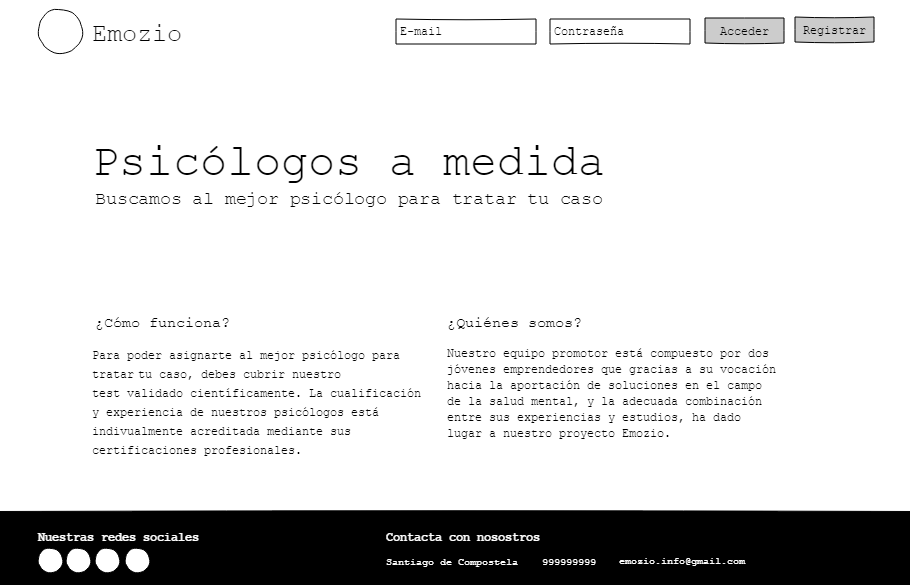
\includegraphics[width=1\textwidth]{figuras/mockup_pacientes/inicio.png}
    \caption{Página de inicio}
    %\label{fig:usn-001}
\end{figure}	

%%%%%%%%%%%%%%%%%%%%%%%%%%%%%%%%%%%%%%%%%%%%%%%%%%%%%%%%%%
%PACIENTES
%%%%%%%%%%%%%%%%%%%%%%%%%%%%%%%%%%%%%%%%%%%%%%%%%%%%%%%%%%

\begin{figure}[htbp] 
    \centering
    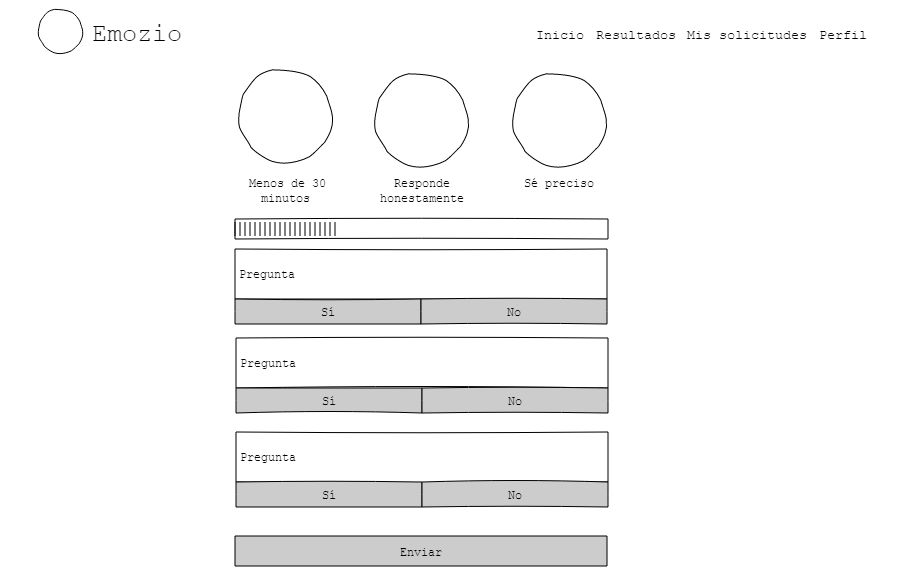
\includegraphics[width=1\textwidth]{figuras/mockup_pacientes/cuestionario.png}
    \caption{Página Cuestionario}
    %\label{fig:usn-001}
\end{figure}	

\begin{figure}[htbp] 
    \centering
    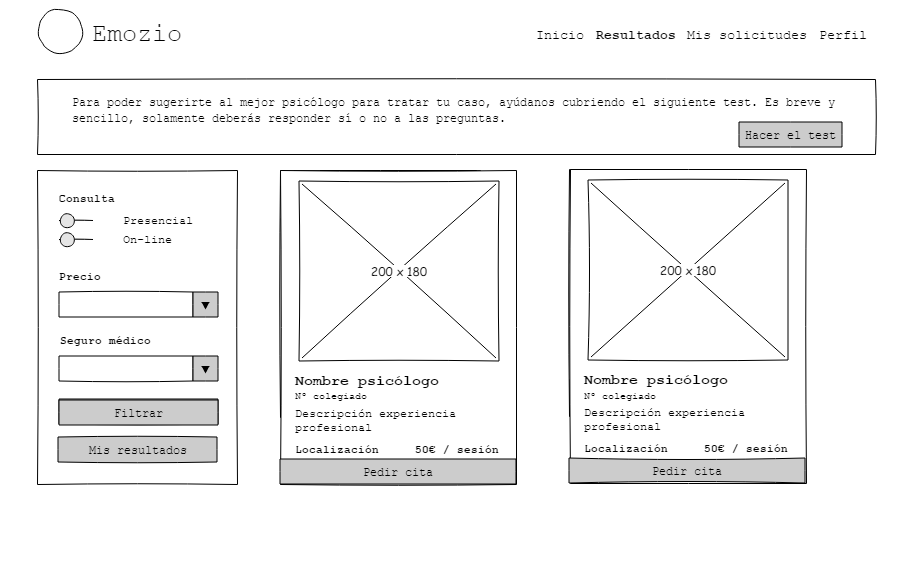
\includegraphics[width=1\textwidth]{figuras/mockup_pacientes/mis_resultados.png}
    \caption{Página Resultados}
    %\label{fig:usn-001}
\end{figure}	

\begin{figure}[htbp] 
    \centering
    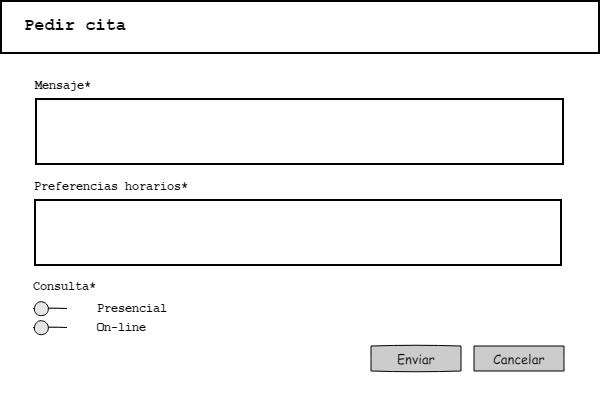
\includegraphics[width=1\textwidth]{figuras/mockup_pacientes/pedir_cita.png}
    \caption{\textit{Pop-up} Pedir cita}
    %\label{fig:usn-001}
\end{figure}	

\begin{figure}[htbp] 
    \centering
    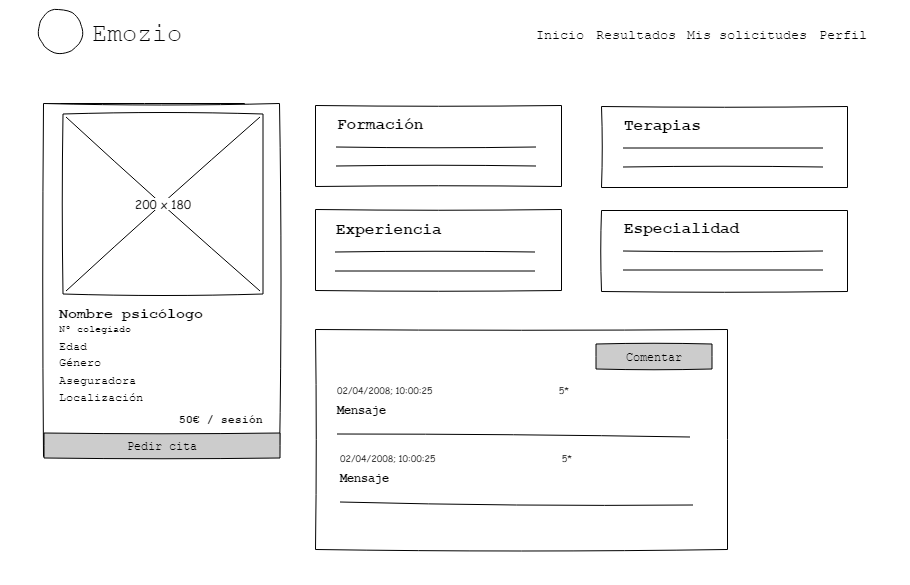
\includegraphics[width=1\textwidth]{figuras/mockup_pacientes/perfil_psicologo.png}
    \caption{Página Perfil psicólogo}
    %\label{fig:usn-001}
\end{figure}	

\begin{figure}[htbp] 
    \centering
    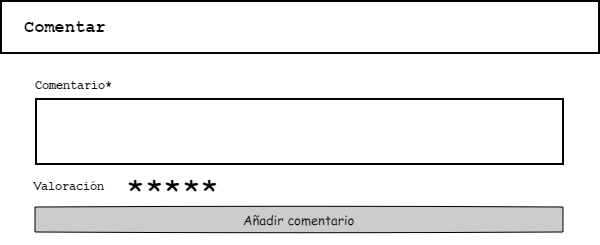
\includegraphics[width=1\textwidth]{figuras/mockup_pacientes/comentar.png}
    \caption{\textit{Pop-up} Comentar}
    %\label{fig:usn-001}
\end{figure}	

\begin{figure}[htbp] 
    \centering
    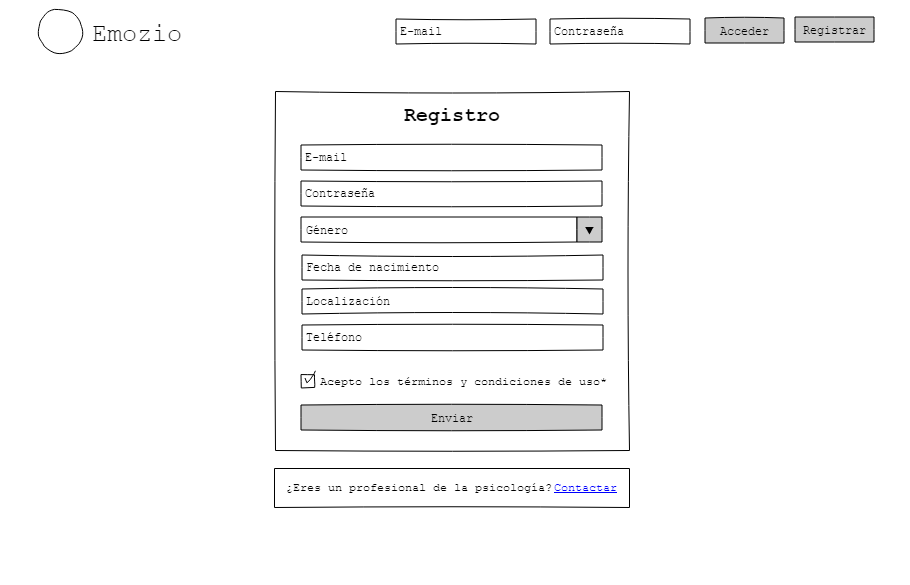
\includegraphics[width=1\textwidth]{figuras/mockup_pacientes/registro.png}
    \caption{Página Registro}
    %\label{fig:usn-001}
\end{figure}	

\begin{figure}[htbp] 
    \centering
    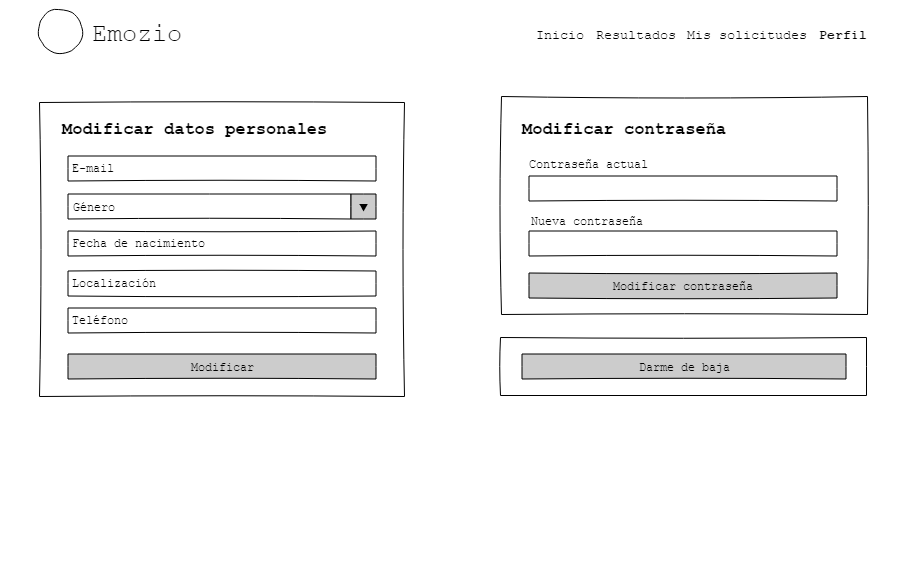
\includegraphics[width=1\textwidth]{figuras/mockup_pacientes/modificar.png}
    \caption{Página Modificar}
    %\label{fig:usn-001}
\end{figure}	

\begin{figure}[htbp] 
    \centering
    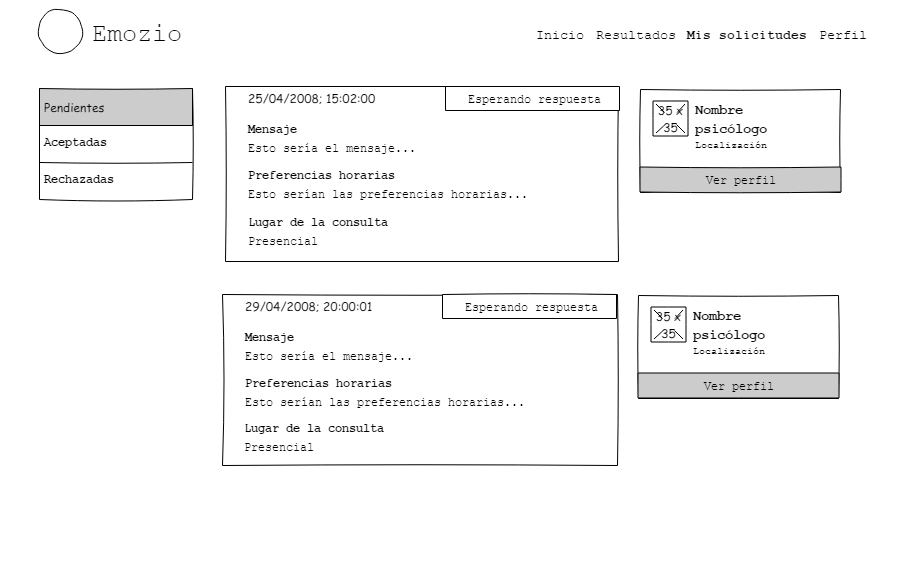
\includegraphics[width=1\textwidth]{figuras/mockup_pacientes/mailpendientes.png}
    \caption{Página Mis solicitudes pendientes}
    %\label{fig:usn-001}
\end{figure}	

\begin{figure}[htbp] 
    \centering
    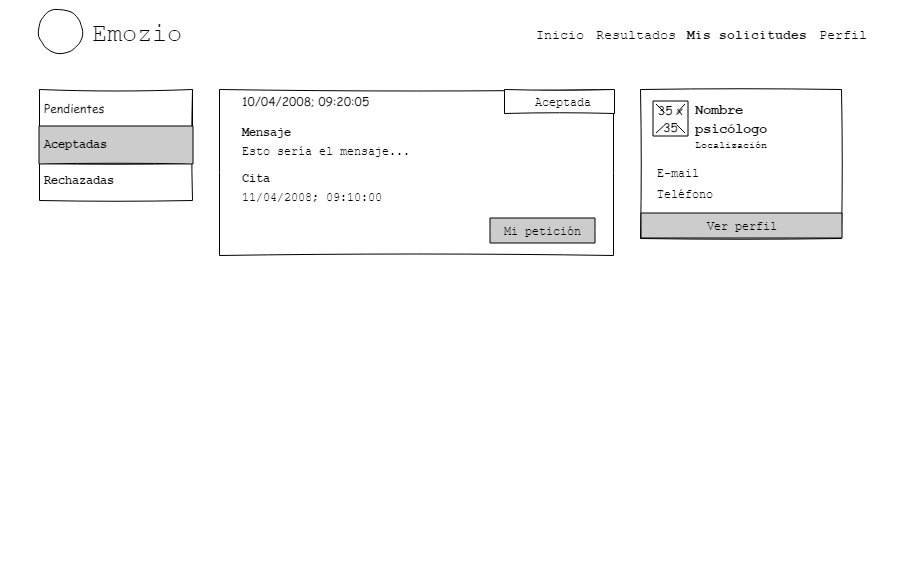
\includegraphics[width=1\textwidth]{figuras/mockup_pacientes/mailaceptadas.png}
    \caption{Página Mis solicitudes aceptadas}
    %\label{fig:usn-001}
\end{figure}	

\begin{figure}[htbp] 
    \centering
    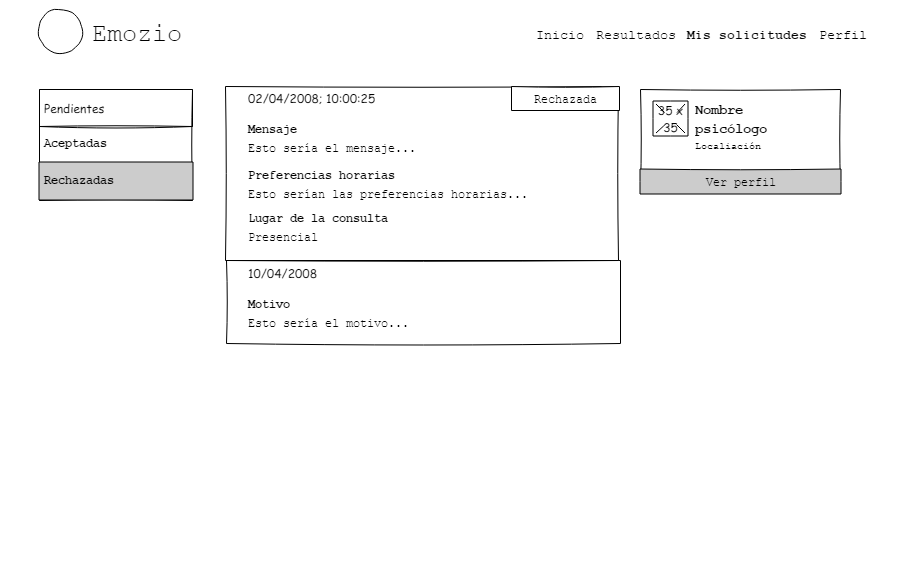
\includegraphics[width=1\textwidth]{figuras/mockup_pacientes/mailrechazadas.png}
    \caption{Página Mis solicitudes rechazadas}
    %\label{fig:usn-001}
\end{figure}	

%%%%%%%%%%%%%%%%%%%%%%%%%%%%%%%%%%%%%%%%%%%%%%%%%%%%%%%%%%
%PSICOLOGOS
%%%%%%%%%%%%%%%%%%%%%%%%%%%%%%%%%%%%%%%%%%%%%%%%%%%%%%%%%%
\begin{figure}[htbp] 
    \centering
    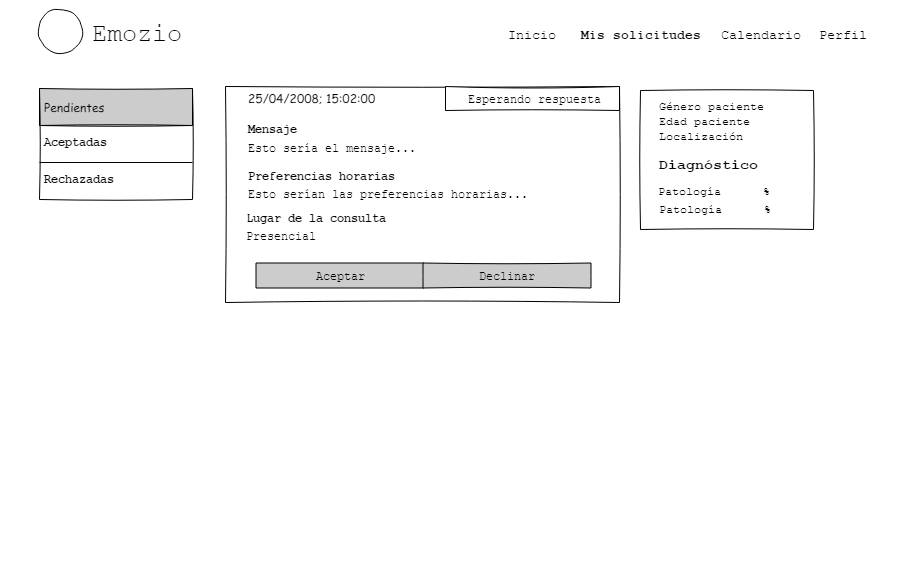
\includegraphics[width=1\textwidth]{figuras/mockup_psicologos/mailpendientes.png}
    \caption{Página Mis solicitudes pendientes}
    %\label{fig:usn-001}
\end{figure}	

\begin{figure}[htbp] 
    \centering
    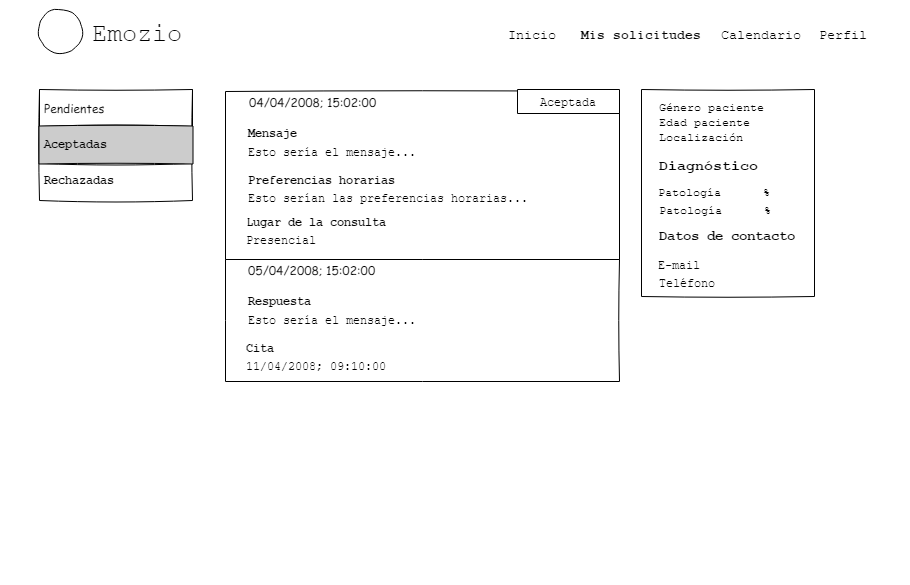
\includegraphics[width=1\textwidth]{figuras/mockup_psicologos/mailaceptadas.png}
    \caption{Página Mis solicitudes aceptadas}
    %\label{fig:usn-001}
\end{figure}	

\begin{figure}[htbp] 
    \centering
    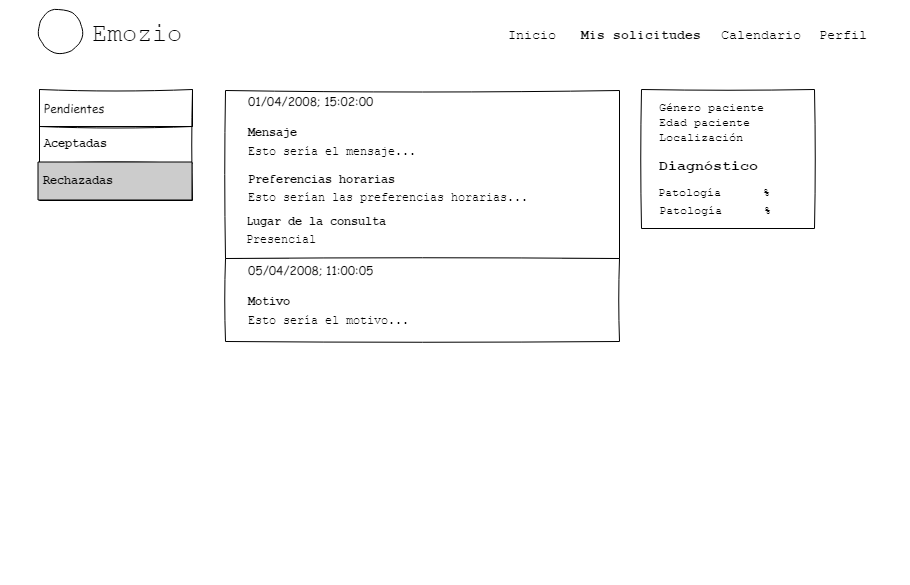
\includegraphics[width=1\textwidth]{figuras/mockup_psicologos/mailrechazadas.png}
    \caption{Página Mis solicitudes rechazadas}
    %\label{fig:usn-001}
\end{figure}	

\begin{figure}[htbp] 
    \centering
    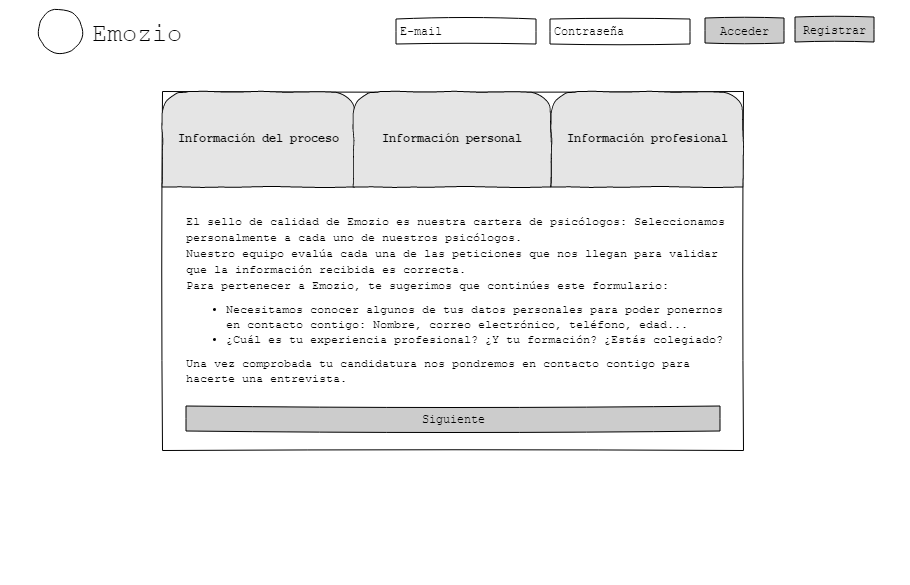
\includegraphics[width=1\textwidth]{figuras/mockup_psicologos/registro1.png}
    \caption{Página Registro Paso 1}
    %\label{fig:usn-001}
\end{figure}	

\begin{figure}[htbp] 
    \centering
    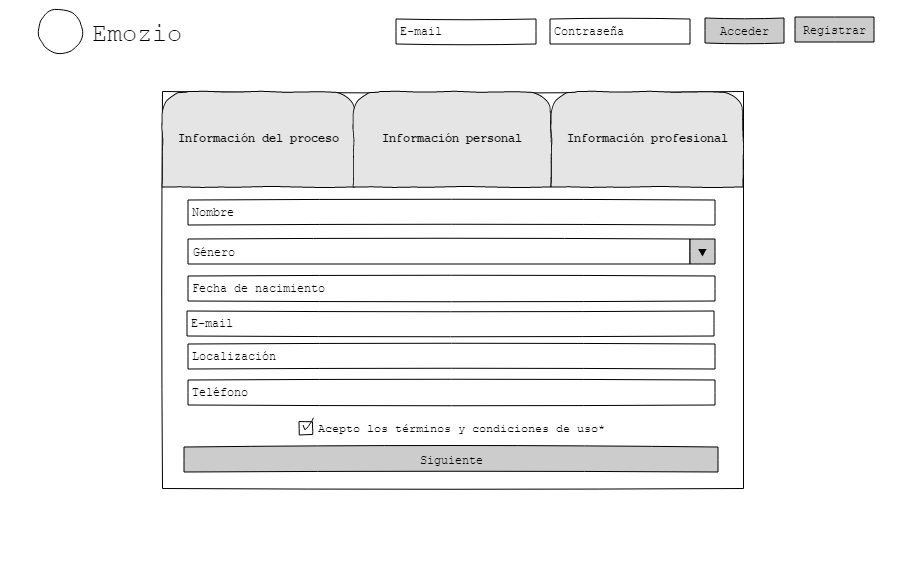
\includegraphics[width=1\textwidth]{figuras/mockup_psicologos/registro2.png}
    \caption{Página Registro Paso 2}
    %\label{fig:usn-001}
\end{figure}	

\begin{figure}[htbp] 
    \centering
    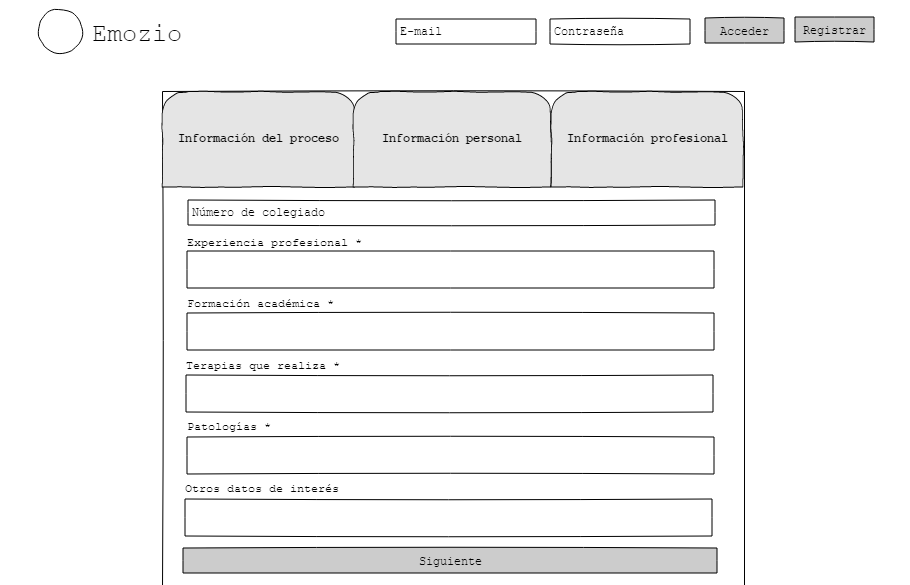
\includegraphics[width=1\textwidth]{figuras/mockup_psicologos/registro3.png}
    \caption{Página Registro Paso 3}
    %\label{fig:usn-001}
\end{figure}	

%%%%%%%%%%%%%%%%%%%%%%%%%%%%%%%%%%%%%%%%%%%%%%%%%%%%%%%%%%%%%%%%%%%%%%%%%%%%%%%%%%%%%%
%%%%%%%%%%%%%%%%%%%%%%%%%%%%%%%%%%%%%%%%%%%%%%%%%%%%%%%%%%%%%%%%%%%%%%%%%%%%%%%%%%%%%%
%DISEÑO DE LA NAVEGACIÓN
%%%%%%%%%%%%%%%%%%%%%%%%%%%%%%%%%%%%%%%%%%%%%%%%%%%%%%%%%%%%%%%%%%%%%%%%%%%%%%%%%%%%%%
%%%%%%%%%%%%%%%%%%%%%%%%%%%%%%%%%%%%%%%%%%%%%%%%%%%%%%%%%%%%%%%%%%%%%%%%%%%%%%%%%%%%%%

\section{Diseño de la navegación}
Para definir las rutas de navegación que permiten a los usuarios acceder al contenido y a las funciones de la plataforma web, debemos identificar la semántica de la navegación para los distintos usuarios del sitio y definir la sintaxis para efectuar la navegación.


\subsection{Semántica de la navegación}
Se define a partir del rol que toma un actor dentro de un caso de uso, ya que cada actor tiene distintos requisitos de navegación. A medida que un usuario interactúa con la web, encuentra una serie de unidades semánticas de navegación (USN) que son un conjunto de estructuras de información y navegación relacionadas que colaboran para el cumplimiento de un subconjunto de requisitos de dicho usuario.


Una USN está compuesta por un conjunto de elementos de navegación llamados formas de navegar (FdN) que representan la mejor ruta de navegación para lograr una meta específica. Está formada por un conjunto de nodos de navegación conectados por vínculos, que en algún pueden tratarse de otra USN.


Para cada caso de uso, se procede a diseñar su USN. Las correspondencias se pueden apreciar en la tabla\ref{cu_usn}.


\begin{table}[htpb]
\centering
\begin{tabular}{|l|l|}
\hline
\rowcolor[gray]{0.9}\textbf{Caso de uso}    & \textbf{Unidad semántica de navegación} \\ \hline
CU-001                  & USN-001 (Paciente)                      \\ \hline
CU-002                  & USN-002                                 \\ \hline
CU-003                  & USN-003                                 \\ \hline
CU-004                  & USN-004                                 \\ \hline
CU-005                  & USN-005                                 \\ \hline
CU-006                  & USN-006                                 \\ \hline
CU-007                  & USN-007                                 \\ \hline
CU-008                  & USN-008                                 \\ \hline
CU-009                  & USN-009                                 \\ \hline
CU-010                  & USN-010                                 \\ \hline
\multirow{2}{*}{CU-011} & USN-011 (Paciente)                      \\ \cline{2-2} 
                        & USN-011 (Psicólogo)                     \\ \hline
CU-012                  & USN-012                                 \\ \hline
\end{tabular}
\caption{Correspondencia entre CU y USN}
\label{cu_usn}
\end{table}

\begin{figure}[htbp] 
    \centering
    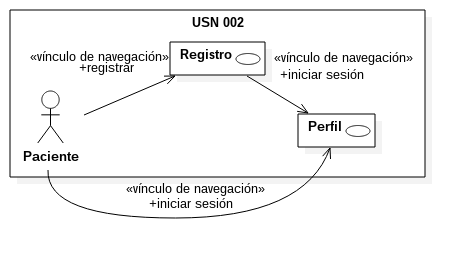
\includegraphics[width=1\textwidth]{figuras/usn/usn001_pac.png}
    \caption{USN-001}
    \label{fig:usn-001}
\end{figure}	

\begin{figure}[htbp] 
    \centering
    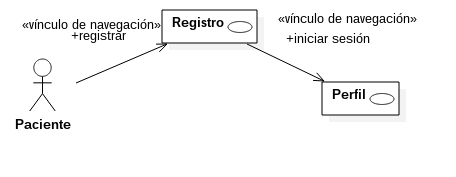
\includegraphics[width=1\textwidth]{figuras/usn/usn002_pac.png}
    \caption{USN-002}
    \label{fig:usn-002}
\end{figure}	

\begin{figure}[htbp] 
    \centering
    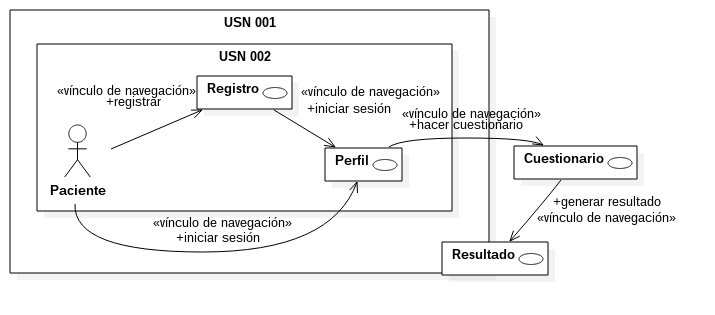
\includegraphics[width=1\textwidth]{figuras/usn/usn003.png}
    \caption{USN-003}
    \label{fig:usn-003}
\end{figure}	

\begin{figure}[htbp] 
    \centering
    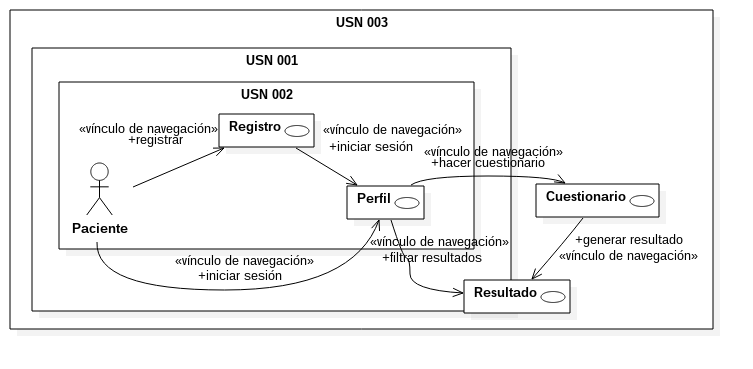
\includegraphics[width=1\textwidth]{figuras/usn/usn004.png}
    \caption{USN-004}
    \label{fig:usn-004}
\end{figure}	

\begin{figure}[htbp] 
    \centering
    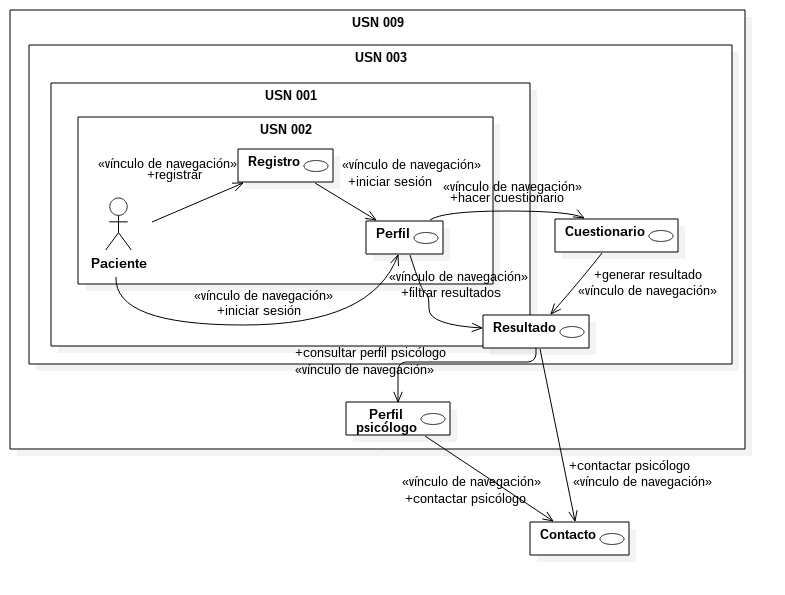
\includegraphics[width=1\textwidth]{figuras/usn/usn005.png}
    \caption{USN-005}
    \label{fig:usn-005}
\end{figure}	

\begin{figure}[htbp] 
    \centering
    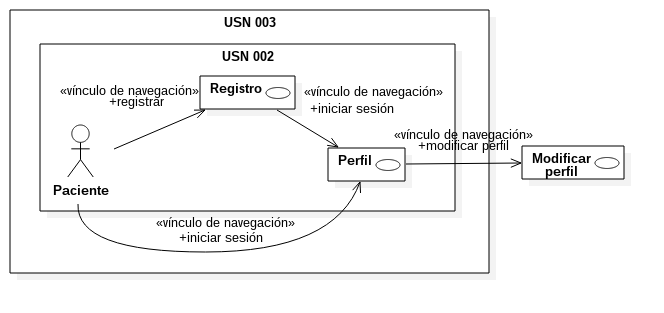
\includegraphics[width=1\textwidth]{figuras/usn/usn006.png}
    \caption{USN-006}
    \label{fig:usn-006}
\end{figure}	

\begin{figure}[htbp] 
    \centering
    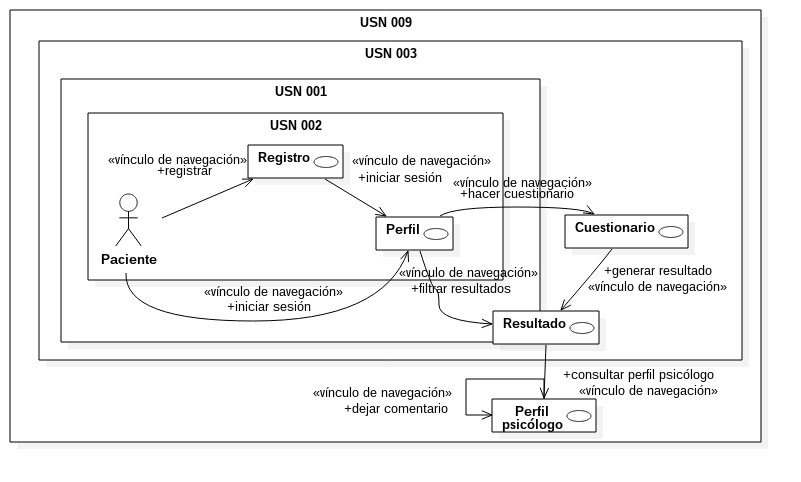
\includegraphics[width=1\textwidth]{figuras/usn/usn007.png}
    \caption{USN-007}
    \label{fig:usn-007}
\end{figure}	

\begin{figure}[htbp] 
    \centering
    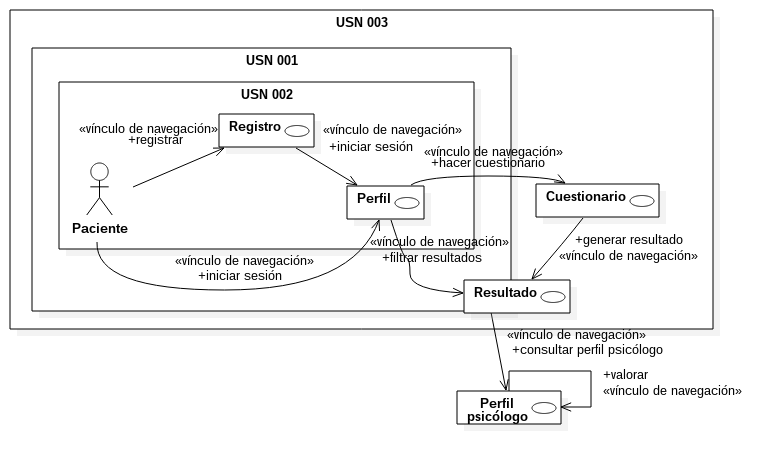
\includegraphics[width=1\textwidth]{figuras/usn/usn008.png}
    \caption{USN-008}
    \label{fig:usn-008}
\end{figure}	

\begin{figure}[htbp] 
    \centering
    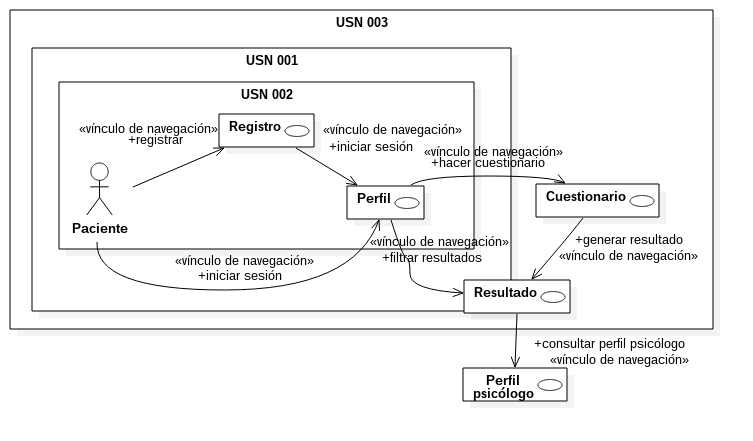
\includegraphics[width=1\textwidth]{figuras/usn/usn009.png}
    \caption{USN-009}
    \label{fig:usn-009}
\end{figure}	

\begin{figure}[htbp] 
    \centering
    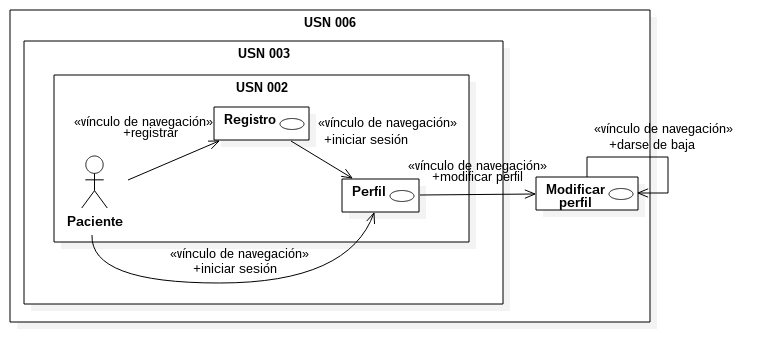
\includegraphics[width=1\textwidth]{figuras/usn/usn010.png}
    \caption{USN-010}
    \label{fig:usn-010}
\end{figure}	

\begin{figure}[htbp] 
    \centering
    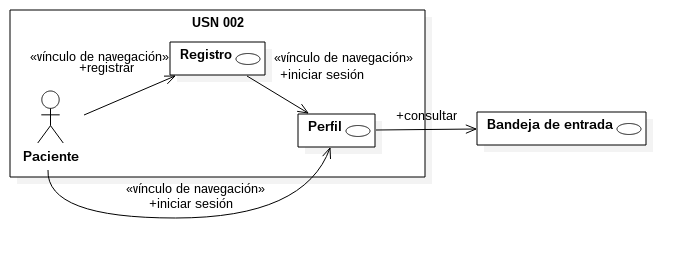
\includegraphics[width=1\textwidth]{figuras/usn/usn011_pac.png}
    \caption{USN-011 (Paciente)}
    \label{fig:usn-011-pac}
\end{figure}	

\begin{figure}[htbp] 
    \centering
    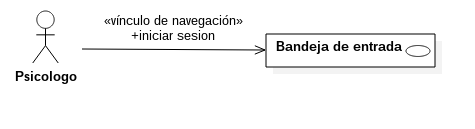
\includegraphics[width=1\textwidth]{figuras/usn/usn011_psic.png}
    \caption{USN-011 (Psicólogo)}
    \label{fig:usn-011-psic}
\end{figure}	

\begin{figure}[htbp] 
    \centering
    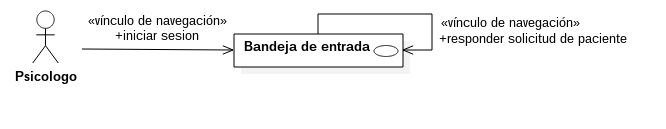
\includegraphics[width=1\textwidth]{figuras/usn/usn012.png}
    \caption{USN-012}
    \label{fig:usn-012}
\end{figure}	

\subsection{Sintaxis de navegación}
La sintaxis de navegación refleja la mecánica de la navegación para cada USN. Para nuestra plataforma web, se ha diseñado un mapa del sitio que describe todas las posibles navegaciones existentes. Para cada tipo de usuario (perfil o psicólogo), existe un mapa\ref{fig:map-nav} diferente.

\begin{figure}[htbp] 
    \centering
    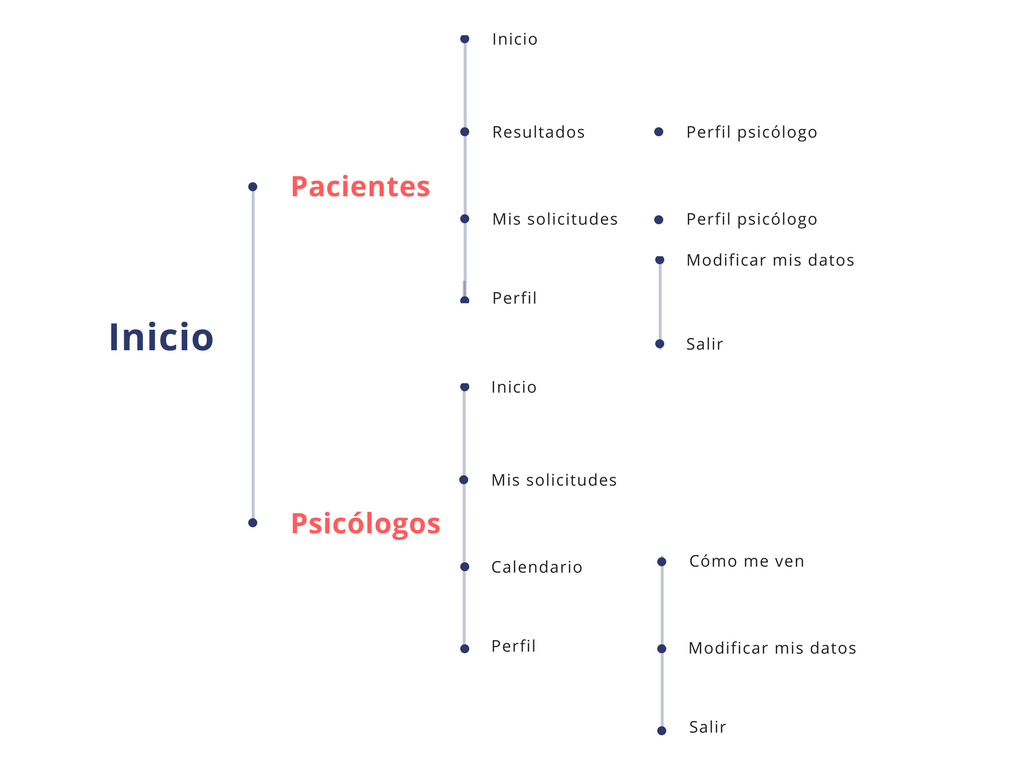
\includegraphics[width=1\textwidth]{figuras/Emozio_Mapa_Navegacion.png}
    \caption{Mapa de navegación}
    \label{fig:map-nav}
\end{figure}	

%%%%%%%%%%%%%%%%%%%%%%%%%%%%%%%%%%%%%%%%%%%%%%%%%%%%%%%%%%%%%%%%%%%%%%%%%%%%%%%%%%%%%%
%%%%%%%%%%%%%%%%%%%%%%%%%%%%%%%%%%%%%%%%%%%%%%%%%%%%%%%%%%%%%%%%%%%%%%%%%%%%%%%%%%%%%%
%TECNOLOGÍAS UTILIZADAS
%%%%%%%%%%%%%%%%%%%%%%%%%%%%%%%%%%%%%%%%%%%%%%%%%%%%%%%%%%%%%%%%%%%%%%%%%%%%%%%%%%%%%%
%%%%%%%%%%%%%%%%%%%%%%%%%%%%%%%%%%%%%%%%%%%%%%%%%%%%%%%%%%%%%%%%%%%%%%%%%%%%%%%%%%%%%%
\section{Tecnologías utilizadas}

\subsection{Frameworks}
Un \textit{framework} es una arquitectura de \textit{software} que modela las relaciones generales de las entidades del dominio, y provee una estructura y una especial metodología de trabajo, la cual extiende o utiliza las aplicaciones del dominio.


Los \textit{frameworks} involucrados en nuestro proyecto son MEAN Stack, Bootstrap y Semantic UI.


\subsubsection{MEAN Stack}
MEAN stack es un \textit{framework} para el desarrollo de aplicaciones, y páginas web dinámicas, basadas en JavaScript: MongoDB, ExpressJS, AngularJS y NodeJS, lo cual permite que se integren entre ellas eficazmente.


Con MongoDB podemos almacenar nuestros documentos en formato JSON, se pueden escribir consultas en nuestro servidor ExpressJS y NodeJS, y del mismo modo, pasar esos documentos JSON a nuestro \textit{frontend} hecho con AngularJS.


El \textit{debugging} y la administración de la base de datos se vuelven más sencillas cuando el objeto almacenado en la base de datos es idéntico al objeto que tu cliente JavaScript puede ver\cite{mongodb_mean_stack}.


Algunos de los motivos por los que escogí este \textit{framework} es por su escalabilidad, rapidez y flexibilidad, ya que permite que en un futuro sea sencillo poder adaptar la aplicación a plataformas móviles, o añadir cambios con facilidad.


Los componentes que forman el \textit{framework} son:


\begin{itemize}
\item \textbf{MongoDB}
MongoDB es una base de datos ágil NoSQL orientada a documentos que permite que los esquemas cambien rápidamente a medida que las aplicaciones evolucionan, proporcionando siempre la funcionalidad que los desarrolladores esperan de las bases de datos tradicionales, tales como índices secundarios, un lenguaje completo de búsquedas y consistencia. En resumen, MongoDB brinda escalabilidad, rendimiento y gran disponibilidad\cite{mongodb_gest_datos}. 
\item \textbf{ExpressJS}
ExpressJS es una middleware de aplicaciones web Node.js minimalista y flexible que proporciona un conjunto sólido de características para aplicaciones web y móviles\cite{express}. Se trata de una API REST que utiliza métodos HTTP para obtener datos o generar operaciones sobre esos datos.
\item \textbf{AngularJS}
AngularJS es un framework para construir client applications en HTML y Javascript, aunque también puede ser otro lenguaje como TypeScript que sea compilado a JavaScript. El framework posee un conjunto de librerías funcionales, y otras opcionales\cite{angular_docs}.


Angular permite fácilmente construir aplicaciones web, ya que combina declarative templates, dependency injection y end to end tooling, e integra buenas prácticas de programación. Las aplicaciones desarrolladas con Angular funcionan tanto para web, móvil o escritorio\cite{angular_arch}. 
\item \textbf{NodeJS}
NodeJS es un entorno de ejecución para JavaScript construido con el motor de JavaScript V8 de Chrome. Node.js usa un modelo de operaciones entrada/salida sin bloqueo (asíncrono) y orientado a eventos, que lo hace liviano y eficiente, ya que nunca se bloquea. 


Node está diseñado sin hilos, este presenta un bucle de eventos como un entorno en vez de una librería. Node simplemente ingresa el bucle de eventos después de ejecutar el \textit{script} de entrada. Node sale del bucle de eventos cuando no hay más callbacks que ejecutar\cite{node_acerca}.
\end{itemize}


\subsubsection{Bootstrap}
Bootstrap es un \textit{framework} de código abierto para desarrollar con HTML, CSS y JS. Contiene características como un grid responsive, docenas de componentes, JavaScript plugins, tipografía, control de formularios y capacidad de personalización\cite{bootstrap}.


\subsubsection{Semantic UI}
Semantic UI es un \textit{framework} que permite a los desarrolladores contruir rápidamente sitios web, con HTML conciso, JavaScript intuitivo, y simplicando el \textit{debugging}. Semantic está diseñado de manera \textit{responsive} permitiendo que la aplicación sea escalable en múltiples dispositivos. Semantic está preparado para poder asociarse con otros frameworks como React, Angular, Meteor y Ember\cite{semantic_github}.


\subsection{Lenguajes de programación}
Los principales lenguajes de programación utilizados son:


\subsubsection{CSS3}
Hojas de Estilo en Cascada (Cascading Style Sheets) es el lenguaje utilizado para describir la presentación de documentos HTML o XML CSS describe como debe ser renderizado el elemento estructurado en pantalla, en papel, hablado o en otros medios\cite{css_mozilla}.


\subsubsection{HTML}
HTML, que significa Lenguaje de Marcado para Hipertextos (HyperText Markup Language) es el elemento de construcción más básico de una página web y se usa para crear y representar visualmente una página web. Determina el contenido de la página web, pero no su funcionalidad\cite{html_mozilla}.


\subsubsection{JavaScript}
Es un lenguaje ligero e interpretado, orientado a objetos con funciones de primera clase, más conocido como el lenguaje de \textit{script} para páginas web, pero también usado en muchos entornos sin navegador, tales como node.js.


Es un lenguaje script multi-paradigma, basado en prototipos\footnote{La programación basada en prototipos es un estilo de programación orientada a objetos que reutiliza comportamientos de objetos existentes.}, dinámico, soporta estilos de programación funcional, orientada a objetos e imperativa\cite{javascript_mozilla}.


\subsection{	\textit{Modules}}
Un \textit{module} es cualquier fichero o directorio que puede ser cargado por NodeJS. 


\subsubsection{Mongoose}
Mongoose proporciona una sencilla, solución basa en esquemas para el modelo de los datos de la aplicación\cite{mongoose}.


\subsubsection{Bcrypt}
Bcrypt permite \textit{hashear} y comparar contraseñas en Node.


\subsubsection{NodeMailer}
NodeMailer permite a las aplicaciones el envío de mensajes.


\subsubsection{FullCalendar}
FullCalendar es un calendario de eventos JavaScript personalizable y de código abierto\cite{fullcalendar}.


\subsection{Librerías}
Una librería es un conjunto de implementaciones funcionales, codificadas en un lenguaje de programación, que ofrece una interfaz bien definida para la funcionalidad que se invoca.


\subsubsection{Places de Google Maps JavaScript API}
Las funciones de la biblioteca JavaScript de Google Places permite que una aplicación busque sitios (definidos en esta API como establecimientos, ubicaciones geográficas o puntos de interés destacados) dentro de un área definida, como los límites de un mapa o alrededor de un punto fijo. También, ofrece una función de autocompletado que puedes usar para dar a tus aplicaciones el comportamiento de escritura anticipada del campo de búsqueda de Google Maps. Cuando un usuario comienza a escribir una dirección, la función de autocompletado termina la tarea\cite{google_api}.


\subsection{	\textit{Middleware}}
Un \textit{middleware} proporciona la lógica de intercambio entre aplicaciones. El \textit{middleware} abstrae de la complejidad y heterogeneidad de las redes de comunicaciones subyacentes, así como de los sistemas operativos y lenguajes de programación, proporcionando una API para la fácil programación y manejo de aplicaciones distribuidas.


\subsubsection{Passport}
Passport es un \textit{middleware} de autenticación para NodeJS. Extremadamente flexible y modular. También puede ser utilizado en cualquier aplicación web basada en Express. Tiene múltiples estrategias que soportan autenticación utilizando nombre y contraseña, Facebook, Twitter, y más\cite{passport}. 


\section{Herramientas utilizadas}
Las herramientas utilizadas en este trabajo fueron:

\begin{itemize}
\item \textbf{Brackets}
\begin{itemize}
\item \textit{Descripción: }Brackets es un editor de texto de código abierto\cite{brackets}.
\item \textit{Uso: }Desarrollo software de la aplicación.
\end{itemize}
\item \textbf{Git}
\begin{itemize}
\item \textit{Descripción: }Git es un sistema de código abierto de control de versiones distribuído diseñado para manipular cualquier tipo de proyectos con rapidez y eficacia\cite{git}.
\item \textit{Uso: }Gestión de la configuración del proyecto.
\end{itemize}
\item \textbf{GitHub}
\begin{itemize}
\item \textit{Descripción: }Es una plataforma de desarrollo colaborativo que permite alojar proyectos utilizando el sistema de control de versiones de Git\cite{github}.  
\item \textit{Uso: }Gestión de la configuración del proyecto.
\end{itemize}
\item \textbf{Grunt}
\begin{itemize}
\item \textit{Descripción: }Es una herramienta que permite simplificar el proceso de construcción (build) de proyectos en JavaScript. Sirven para automatizar tareas repetitivas como minificación, compilación, testeo unitario...\cite{grunt}
\item \textit{Uso: }Durante el desarrollo de la aplicación.
\end{itemize}
\item \textbf{\LaTeX}
\begin{itemize}
\item \textit{Descripción: }Es un sistema tipográfico que incluye características diseñadas para la producción de documentación técnica y científica\cite{latex}.
\item \textit{Uso: }Elaboración de la memoria final.
\end{itemize}
\item \textbf{LibreOffice}
\begin{itemize}
\item \textit{Descripción: }Es un conjunto de aplicaciones de oficina: Writer, el procesador de textos, Calc, la hoja de cálculos, Impress, el editor de presentaciones, Draw, nuestra aplicación de dibujo y diagramas de flujo; entre otros\cite{libreoffice}. 
\item \textit{Uso: }Borradores y algunos diagramas del proyecto.
\end{itemize}
\item \textbf{Pencil}
\begin{itemize}
\item \textit{Descripción: }Pencil es una GUI de prototipado de código abierlo para creación de \textit{mockups}\cite{pencil}.
\item \textit{Uso: }Elaboración del \textit{mockup}.
\end{itemize}
\item \textbf{NPM}
\begin{itemize}
\item \textit{Descripción: }NPM es un gestor de paquetes JavaScript. Es el repositorio más grande de librerías de código abierto en el mundo\cite{npm}. 
\item \textit{Uso: }Instalación de paquetes y librerías software.
\end{itemize}
\item \textbf{Robomongo}
\begin{itemize}
\item \textit{Descripción: }Robomongo es una GUI que maneja la shell de MongoDB\cite{robomongo}.
\item \textit{Uso: }Gestión de la base de datos.
\end{itemize}
\item \textbf{StarUML}
\begin{itemize}
\item \textit{Descripción: }StarUML es una herramienta de modelado UML que permite hacer multitud de tipos de diagramas como de clase, de objeto, de casos de uso, de componente, entre otros\cite{staruml}. 
\item \textit{Uso: }Diseño de los diagramas del proyecto.
\end{itemize}
\end{itemize}

%%%%%%%%%%%%%%%%%%%%%%%%%%%%%%%%%%%%%%%%%%%%%%%%%%%%%%%%%%%%%%%%%%%%%%%%%%%%%%%%%%%%%%
%%%%%%%%%%%%%%%%%%%%%%%%%%%%%%%%%%%%%%%%%%%%%%%%%%%%%%%%%%%%%%%%%%%%%%%%%%%%%%%%%%%%%%
%SEGURIDAD
%%%%%%%%%%%%%%%%%%%%%%%%%%%%%%%%%%%%%%%%%%%%%%%%%%%%%%%%%%%%%%%%%%%%%%%%%%%%%%%%%%%%%%
%%%%%%%%%%%%%%%%%%%%%%%%%%%%%%%%%%%%%%%%%%%%%%%%%%%%%%%%%%%%%%%%%%%%%%%%%%%%%%%%%%%%%%
\section{Seguridad}
\subsection{¿Qué es Bcrypt?}
Niels Provos y David Maxieres diseñaron Bcrypt, una función de \textit{hashing} de contraseñas basado en el tipo de cifrado Blowfish. Es empleado en algunas distribuciones de Linux por defecto. 


Cuando se genera un \textit{hash} asociado a la contraseña por lo general los algoritmos comunes (md5, sha-1,…) incorporan un valor de \textit{salt}, este fragmento se emplea para generar dicho \textit{hash}, de esta forma se consigue que dos contraseñas iguales que generarían el mismo \textit{hash} no lo hagan, algo muy importante para luchar contra ataques de fuerza bruta, así como para dificultar los ataques de Rainbow table.


Los ataque de Rainbow table son efectivos cuando las contraseñas son ``hasheadas'' de la misma manera, de esta forma para dos contraseñas iguales el hash sería el mismo. Así es como surge el \textit{salt}, añadir un \textit{hash} a cada contraseña nos devuelve dos \textit{hashes} distintos para la misma contraseña. Es importante evitar la \textit{reutilización} de \textit{salt}. Sin embargo no es suficiente el uso de \textit{salt} para el almacenamiento de contraseñas debido a que \textit{salt} pasa a ser inútil para ataques de fuerza bruta o de diccionario.


\subsection{Ventajas de Bcrypt}
En este punto es donde entra Bcrypt, para solucionar el problema en el que nos hallamos debemos hablar del número de iteraciones. Esto mejora a los \textit{hashes} comunes gracias a su lentitud. ¿Qué quiere decir esto? Empleando una variante de cifrado Blowfish se introduce un factor de trabajo que permite controlar el coste de la función \textit{hash}. Mediante este factor Bcrypt se actualiza de acuerdo a la ley de Moore con la evolución de la tecnología.


Para verlo más concretamente podemos ver la tabla de comparación siguiente, y recalcar que aunque las contraseñas no requieran de una protección tan elevada, gracias al factor de trabajo la optimización de bcrypt se consigue con un buen equilibrio entre velocidad y seguridad. El sacrificio de un poco de rendimiento se traduce en un aumento de la seguridad. 
Esta tabla muestra una prueba de la fuerza de bcrypt, que ha sido lanzado en un clúster de 25 GPU para la rotura de contraseñas en \textit{hash}, han resultado los siguientes datos:


\begin{itemize}
\item md5(\$password) 
\begin{itemize}
\item 180 billones resultados/s
\item 9.4 Horas
\end{itemize}
\item sha1(\$password)
\begin{itemize}
\item 61 billones resultados/s
\item 27 Horas
\end{itemize}
\item md5crypt
\begin{itemize}
\item 77 millones resultados/s
\item 2.5 Años
\end{itemize}
\item bcrypt con un factor de 5 
\begin{itemize}
\item 71 mil resultados/s
\item 2700 Años
\end{itemize}
\end{itemize}


\subsection{Funcionamiento}
La librería bcrypt nos permite crear el \textit{hash} de una contraseña mediante \textit{saltRounds}, este valor nos da control sobre el factor de coste de procesado de datos. A mayor valor de \textit{saltRound} mayor coste de cálculo del \textit{hash} asociado a una contraseña.  Por defecto este valor viene situado en 10. 


En el caso del registro de usuario se envía la contraseña y el valor del parámetro \textit{saltRounds} a la librería para que la cifre, esta nos devuelve el \textit{hash} asociado a la contraseña en el usuario de la base de datos. Cuando el usuario quiere entrar la contraseña introducida se cifra, para ello se busca el \textit{salt} asociado al usuario de la base de datos. Una vez cifrada con el \textit{salt} se comparan los \textit{hashes}. La librería nos devuelve un booleano que indica si las contraseñas coinciden o no, con lo cual podemos dejar entrar el usuario o devolver un error.


\subsection{Cifrado Blowfish}
Bruce Schneier en 1993 diseña un codificador de bloques simétricos de 64 bits, con claves de hasta 448 bits, es empleado en un abundante número de productos de cifrado. No tiene técnicas de criptoanálisis que hayan resultado efectivas contra este algoritmo. Su licencia es totalmente libre.


%%%%%%%%%%%%%%%%%%%%%%%%%%%%%%%%%%%%%%%%%%%%%%%%%%%%%%%%%%%%%%%%%%%%%%%%%%%%%%%%%%%%%%
%%%%%%%%%%%%%%%%%%%%%%%%%%%%%%%%%%%%%%%%%%%%%%%%%%%%%%%%%%%%%%%%%%%%%%%%%%%%%%%%%%%%%%
%DISEÑO DE LA ARQUITECTURA
%%%%%%%%%%%%%%%%%%%%%%%%%%%%%%%%%%%%%%%%%%%%%%%%%%%%%%%%%%%%%%%%%%%%%%%%%%%%%%%%%%%%%%
%%%%%%%%%%%%%%%%%%%%%%%%%%%%%%%%%%%%%%%%%%%%%%%%%%%%%%%%%%%%%%%%%%%%%%%%%%%%%%%%%%%%%%
\section{Diseño de la arquitectura}

\subsection{	\textit{Single page aplication}}
\textit{Single page aplication}, de ahora en adelante SPA, es una aplicación o sitio web que cabe en una sóla página web con el objeto de proveer una experiencia de usuario más fluida y una interfaz más enriquecida. Una de las ventajas de este tipo de aplicaciones es que son capaces de actualizar una parte de la interfaz, sin necesidad de enviar o recibir una petición de \textit{full-page}\cite{fernandomonteiro2014}.


\subsection{Particularidades de JavaScript}
\subsubsection{En JavaSCript no existen las clases}
JavaScript es un lenguaje orientado a objetos basado en prototipos en lugar de clases. A diferencia de los lenguajes orientados a objetos basados en clases, un lenguaje basado en prototipos no hace distinción entre clases e instancias: Simplemente tiene objetos. Estos objetos son conocidos como objetos prototípicos, que son objetos que se utilizan como una plantilla a partir de la cual se obtiene el conjunto inicial de propiedades de un nuevo objeto\cite{fernandomonteiro2014}.


Para poder entender cuáles son las diferencias entre un lenguaje orientado a objetos basados en clases (Java) y basados en prototipos (JavaScript) se han listado sus diferencias en la tabla \ref{java-js}.


\begin{table}[htpb]
\centering
\begin{tabularx}{\textwidth}{|X|X|}
\hline
\rowcolor[gray]{0.9}\textbf{Basados en clases (Java)}                                                                                                                                       & \textbf{Basados en prototipos (JavaScript)}                                                                                                                                                  \\ \hline
La clase y su instancia son entidades distintas                                                                                                                         & Todos los objetos pueden heredar de otro objeto                                                                                                                                              \\ \hline
Define una clase en la definición de clase; se instancia una clase con los métodos constructores.                                                                       & Define y crea un conjunto de objetos con funciones constructoras.                                                                                                                            \\ \hline
Se crea un objeto con el operador new.                                                                                                                                  & Igual.                                                                                                                                                                                       \\ \hline
Se construye una jerarquía de objetos utilizando la definición de las clases para definir subclases de clases existentes.                                               & Se construye una jerarquía de objetos mediante la asignación de un objeto como el prototipo asociado a una función constructor.                                                              \\ \hline
Se heredan propiedades siguiendo la cadena de clases.                                                                                                                   & Se heredan propiedades siguiendo la cadena de prototipos.                                                                                                                                    \\ \hline
La definición de una clase especifica todas las propiedades de todas las instancias de esa clase. No se pueden añadir propiedades dinámicamente en tiempo de ejecución. & El conjunto inicial de propiedades lo determina la función constructor o el prototipo. Se pueden añadir y quitar propiedades dinámicamente a objetos específicos o a un conjunto de objetos. \\ \hline
\end{tabularx}
\caption{Comparativa Java y JavaScript}
\label{java-js}
\end{table}


Por estos motivos, los patrones que se han diseñado con UML consisten en una aproximación de cómo se representaría el diseño de la plataforma.


\subsection{	\textit{Callbacks} en JavaScript}
Las \textit{callbacks} JavaScript son utilizadas para gestionar eventos de manera responsable en el lado cliente ejecutando funciones asíncronas, y en Node, las \textit{callbacks} también son utilizadas en el lado servidor para dar servicio a múltiples peticiones simultáneas de clientes.


Una \textit{callback} es una función que es pasada como argumento a otra función, que espera ser invocada tanto inmediátamente como en algún momento futuro.


Las \textit{callbacks} pueden ser vistas como una forma de ``\textit{continuation-passing style}'' (CPS), cuyo control es pasado explícitamente de forma continuada, en el caso de las \textit{callback} es pasado como argumento representando una continuación.


JavaScript utiliza un modelo \textit{event-driven} con un único hilo de ejecución. Programar con \textit{callbacks} es especialmente útil cuando el llamador no quiere esperar hasta que la llamada se complete. Para conseguirlo, la operación no bloqueante (\textit{non-blocking operation}) es agendada (\textit{scheduled}) como una \textit{callback} y el hilo principal continua su síncrona ejecución. Cuando la operación se completa, un mensaje es encolado en una cola de tareas según la \textit{callback} que lo provee. El bucle de eventos (\textit{event loop}) en JavaScript prioriza que el hilo ejecute la pila de llamadas primero; cuando la pila está vacía, el bucle de eventos desencola un mensaje para la cola de tareas y ejecuta la correspondiente función \textit{callback}.
En JavaScript, las \textit{callbacks} pueden llamarse ``funciones'' o ``funciones anónimas''.
En el proyecto, para gestionar las \textit{callbacks} se han utilizado promises. Las \textit{promise} son una extensión del lenguaje JavaScript \cite{keheliyagallabaalimesbahivanbeschastnikh2015}.


Una \textit{promise} es un \textit{proxy} para un valor no necesariamente conocido en el momento que es creada. Permite asociar manejadores que actuarán asincrónicamente sobre un eventual valor en caso de éxito, o la razón del fallo. Esto permite que métodos asíncronos devuelvan valores como si fueran síncronos: en vez de inmediatamente retornar el valor final, el método asíncrono devuelve una \textit{promise} y suministra su valor en algún momento en el futuro\cite{promise_objeto}. Al objeto le enganchas las funciones \textit{callback}, en vez de pasar funciones \textit{callback} a una función\cite{promise_mozilla}. Nos permiten mejorar la legibilidad de nuestro código y evitar tener que pasar el contenido de las funciones directamente como argumentos a nuestra llamada. Las \textit{promise} en JavaScript sirven para evitar el ``\textit{callback-hell}'' que surge de llamar a una función asíncrona en JavaScript. 


\subsubsection{Implementando patrones de diseño con JavaScript}
En la mayoría de lenguajes tradicionales orientados a objetos existen las clases, las interfaces, la herencia, la encapsulación y el polimorfismo. Pero JavaScript, no, puesto que es muy sencillo: Trabaja por medio de callbacks (funciones).


Un objeto es la unidad responsable de proporcionar estados y comportamiento; y la declaración de las funciones en JavaScript proporcionan ambas\cite{angular_embrace}.


\subsection{Patrones de diseño}
\subsubsection{MVC y MVVM}
El patrón Modelo Vista Controlador, de ahora en adelante MVC, es un patrón de arquitectura software que permite separar la representación visual de la información, de la interacción del usuario. 


MVC es un patrón \textit{composite}. Los patrones \textit{composite} son aquellos patrones capaces de trabajar juntos para darle solución a un problema en común\cite{ericfreemanelisabethfreemanbertbates2004}. 


El patrón de diseño MVC está compuesto por:


\begin{itemize}
\item Modelo: Almacena toda la información, estados y lógica de la aplicación.
\item Vista: Se trata de a interfaz de usuario que muestra una representación del modelo. La vista informa al controlador qué trata de hacer el usuario. 
\item Controlador: Toma la entrada del usuario, la gestiona y le transmite lo que ha interpretado al modelo. También, manipula cómo se debe ver la vista.
\end{itemize}


Actualmente, se han desarrollado nuevos tipos de modelo MV*, como el Modelo Vista VistaModelo, de ahora en adelante MVVM, que está basada en el patrón MVC y el Modelo Vista Presentador, que trata de separar con más claridad el desarrollo de la interfaz de usuario con el de la lógica de negocio y el comportamiento de la aplicación.


Los componentes de los patrones MVVM son:


\begin{itemize}
\item Modelo: Representa los datos específicos del dominio o información con la que nuestra aplicación debe trabajar. Almacena información, pero comúnmente no posee ningún tipo de comportamiento. No formatean la información ni influencian en cómo los datos aparecen en el navegador, ya que no es su responsabilidad.
\item Vista: Es la única parte de la aplicación con la que el usuario interactúa. Contiene la información obtenida de la sincronización entre la vista y el modelo (\textit{data binding}\cite{data_binding_w3s}), los eventos y comportamientos. Es una interfaz de usuario interactiva que representa el estado de la VistaModelo. La vista no es la encargada de gestionar su estado, sólo se mantiene sincronizada con la VistaModelo.
\item VistaModelo: Se puede considerar como un Controlador especializado que actúa como un conversor de datos. Transforma la información del Modelo en la información de la Vista\cite{fernandomonteiro2014}. 
\end{itemize}

En MEAN STACK, estos dos patrones se pueden aparecen combinados como se muestra en la figura\ref{fig:mvc_mvvm}.


\begin{figure}[htbp] 
    \centering
    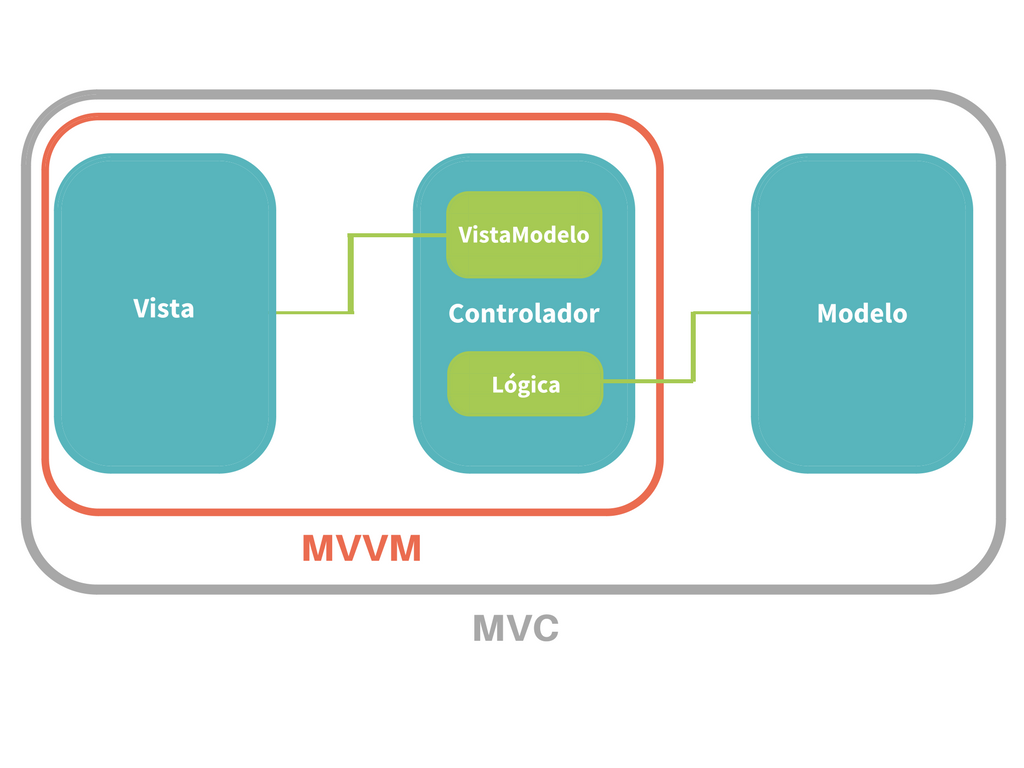
\includegraphics[width=1\textwidth]{figuras/MVC_MVVM.png}
    \caption{Mean STACK - MVC y MVVM}
    \label{fig:mvc_mvvm}
\end{figure}	


\subsubsection{\textit{Page Controller}}
\textit{Page Controller} tiene un único \textit{controller} por cada página lógica de la página web\cite{martinfowler2002}.


Las responsabilidades del \textit{Page Controller} son:


\begin{itemize}
\item Analizar la URL y extraer cualquier dato de formulario necesario para el comportamiento.
\item Crear e invocar cualquier objeto del modelo para procesar datos. Cualquier dato relevante de una petición HTML ha de ser pasada al modelo, de esta forma el modelo no necesita ningún tipo de conexión a las peticiones HTML.
\item Determina qué vista ha de ser mostrada a continuación como resultado de la página y proporcionar al modelo información sobre ello.
\end{itemize}


El patrón \textit{Page Controller} acepta entradas desde la petición de una página, invoca las acciones pedidas en el modelo, y determina la vista que se ha de usar como página resultante\cite{page_controller_microsoft}.


En AngularJS, tenemos \textit{controllers} los cuales tienen unas responsabilidades limitadas: Ellos no aceptan las peticiones del usuario porque es la responsabilidad de los \textit{services} \$route o \$state y la renderización de la página es responsabilidad de la directiva ng-view. Para determinar qué vista ha de ser mostrada utiliza el \textit{service} \$location.


Al igual que \textit{page controllers}, los \textit{controllers} de AngularJS gestionan las interacciones de usuario, proveen y actualizan los modelos. El modelo está unido a la vista a través de \$scope\cite{mgechev}.


\subsection{	\textit{Observer}}
El patrón \textit{Observer} es un patrón de diseño \textit{software} en el cual un objeto, llamado \textit{subject}, mantiene una lista de sus dependencias, llamadas \textit{observers}, y las notifica automáticamente en cualquier cambio de estado, normalmente utilizando uno de sus métodos. 


\subsubsection{\textit{Data-binding}}
\textit{Data binding} en Angular es la sincronización entre el modelo y la vista.


El \textit{controller} proporciona comportamiento a través de \$scope, mientras que {{}} se pueden utilizar en el código HTML para mostrar contenido del modelo en la vista. O la \textit{directive} ng-model para asociar el modelo con la vista.


Cuando la información en el modelo cambia, la vista refleja dicho cambio, y cuando la vista es modificada, el modelo se actualiza.


Debida a la inmediata sincronización entre el modelo y la vista, el controlador puede estar completamente separado de la vista, y simplemente concentrarse en el modelo de datos\cite{data_binding_w3s}.


El mostrado en la figura \ref{fig:data_binding} representa el funcionamiento descrito a continuación. El \textit{module} es el objeto de mayor nivel en Angular. Una aplicación Angular es especificada por la directiva ng-app siempre correspondiente a un módulo.
Config es un objeto que configura la aplicación Angular, permite configurar las rutas (\textit{routes}) necesarias en la SPA porque gestionan las \textit{templates}. En Angular se empareja cada \textit{template} con un \textit{controller}. La <view> representa la parte \textit{front-end} y el \textit{controller} y la \textit{factory}  representan el \textit{back-end}. \$scope vive entre ambos, y Angular permite asegurar que ambos tengan la última versión de la aplicación. El bucle de eventos y \$scope permiten a Angular \textit{two way data binding}, y como resultado es que ya no es necesario acceder al DOM desde JavaScript\cite{paislee}.   


\begin{figure}[htbp] 
    \centering
    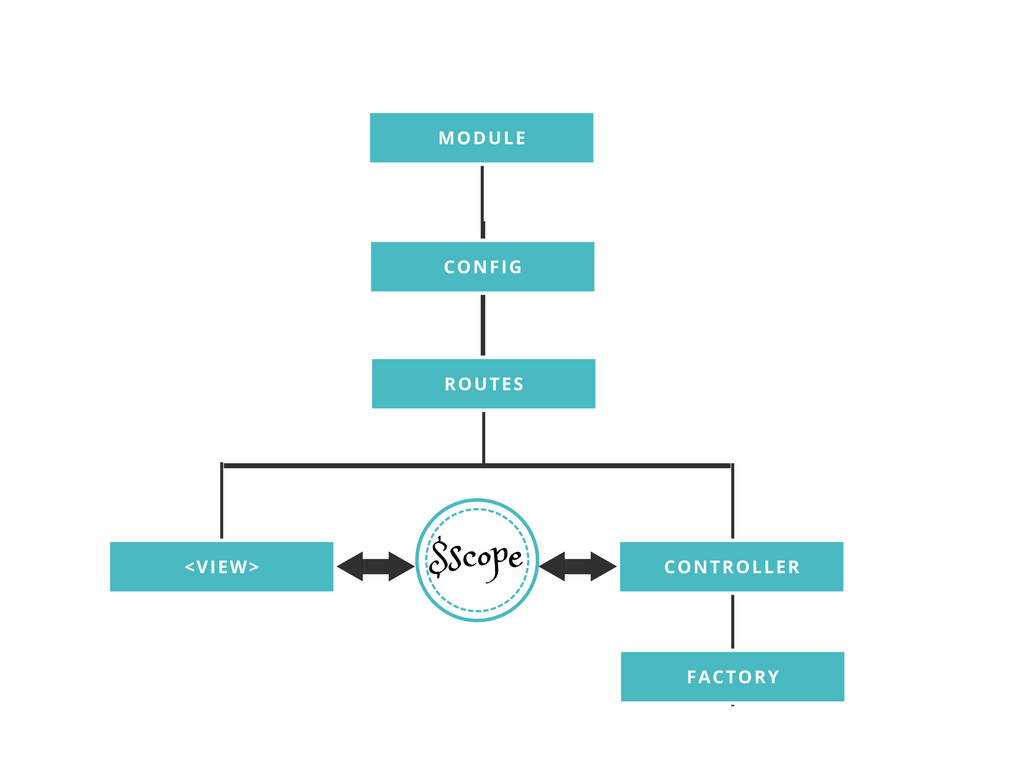
\includegraphics[width=1\textwidth]{figuras/data_binding.png}
    \caption{Esquema \textit{data-binding}}
    \label{fig:data_binding}
\end{figure}	


\subsubsection{\textit{Dependency Injection}}
\textit{Dependency injection} permite obtener una instancia de las clases que se requieren y que una \textit{factory} o \textit{injector} te las provea tanto en tiempo de compilación como en el de ejecución\cite{depend_inject}.


\textit{Dependency injection} suele ser utilizado para evitar al patrón \textit{Singleton}\cite{mgechev}.


\subsection{\textit{Factory Method}}
Los propósitos del patrón \textit{Factory} son:


\begin{itemize}
\item Crear objetos
\item Realiza operaciones repetitivas cuando se preparan objetos similares.
\item Ofrece que los consumidores de la \textit{Factory} puedan crear objetos sin necesidad de conocer el tipo específico (de la clase) en tiempo de compilación\cite{stoyanstefanov2010}.
\end{itemize}


El patrón \textit{factory} provee una interfaz genérica para crear objetos, donde hay que especificar el tipo de objeto \textit{factory} que deseamos obtener\cite{addyosmani2012}.


En AngularJS se hace por medio del \textit{Factory Method}\cite{mgechev}.


\subsection{	\textit{Proxy}}
En el patrón \textit{proxy}, un objeto actúa como interfaz de otro objeto. El \textit{proxy} se encuentra entre el cliente de un objeto y el objeto en sí, protegiendo el acceso a dicho objeto.


Al tratarse de un \textit{proxy} virtual solventa la problemática que existe si inicializar el sujeto real es costoso, y puede ocurrir que el cliente lo inicialice pero nunca llegue a usarlo. En este caso, el \textit{proxy} puede ayudar siendo la interfaz del sujeto real. El \textit{proxy} recibe la petición de inicialización, pero nunca lo pasa a no ser que realmente el sujeto real sea utilizado. 


La imagen \ref{fig:proxy}, muestra el posible escenario de cuando un cliente realiza una petición de inicialización y el \textit{proxy} responde que todo está bien, pero realmente no pasa el mensaje, a no ser que sea obvio que el cliente necesite hacer algo con el sujeto. Sólo en ese caso, el \textit{proxy} le pasará ambos mensajes juntos\cite{stoyanstefanov2010}.
 

\begin{figure}[htbp] 
    \centering
    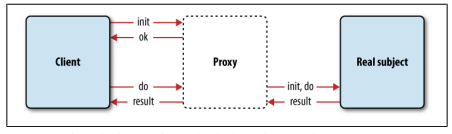
\includegraphics[width=1\textwidth]{figuras/proxy_pattern.png}
    \caption{\textit{Proxy pattern}\cite{stoyanstefanov2010}}
    \label{fig:proxy}
\end{figure}	


\subsection{\textit{Data Mapper}}
Un \textit{Data Mapper} es una capa de acceso a datos (\textit{Data Access Layer}) que permite la transferencia bidireccional de datos entre el lugar de almacenamiento de los datos persistentes y la representación en memoria de esos datos, manteniéndolos independientes\cite{mgechev}.


En Angular a través del módulo ngResource, nos permite realizar conexiones REST a nuestra API para enviar y recibir información mediante el servicio \$http. Sin embargo, los datos pasados desde el servidor se encuentran en un formato apropiado gracias a la librería Mongoose.


Mongoose proporciona por un lado el esquema que da formato a los datos obtenidos de la base de datos, y por otro lado, el acceso a los mismos. 


\subsection{API REST}
REST (\textit{Representational State Transfer}) es un estilo de arquitectura diseñado para sistemas distribuídos. No está estandarizado pero posee una serie de directivas, como permanecer sin estado, tener relaciones cliente-servidor y una interfaz uniforme. Suele estar relacionado con HTTP.


Sus principios son:


\begin{itemize}
\item Expone recursos fácilmente con un directorio de URLs estructurado.
\item Representa los data objects y atributos en formato JSON o XML.
\item Los mensajes utilizan métodos HTTP explícitamente: GET, POST, PUT y DELETE.
\item Protocolo cliente/servidor sin estado: Cada petición HTTP contiene toda la información necesaria para ejecutarla, lo que permite que ni cliente ni servidor necesiten recordar ningún estado previo para satisfacerla\cite{rest_spring}.
\end{itemize}


\subsection{Estructura de directorios}
Es importante mantener una estructura de directorios\ref{fig:directorios} y de código organizada, pensando en el mantenimiento y en la escalabilidad de la aplicación. 


A continuación, se describen (por orden de aparición) los distintos directorios y ficheros que pertenecen a la estructura básica del proyecto:


\begin{itemize}
\item \texttt{app}
Contiene la parte \textit{frontend} de la aplicación.
\item \texttt{assets}
Contiene algunos de los recursos de la aplicación.
\item \texttt{images}
Contiene las imágenes utilizadas en la aplicación.
\item \texttt{javascript}
Contiene todos los archivos JavaScript de la parte \textit{frontend} de la aplicación.
\item \texttt{app.js}
Es nuestro fichero de inicio.
\item \texttt{controllers}
Contiene los \textit{controllers} de los \textit{templates}.
\item \texttt{routes.js}
Archivo que determina el enrutado de nuestra aplicación.
\item \texttt{factories}
Contiene los \textit{factories}.
\item \texttt{vendor}
Contiene algunas librerías JavaScript utilizadas en la aplicación.
\item \texttt{semantic}
Contiene todos los archivos del paquete semantic-ui.
\item \texttt{styles}
Contiene algunas librerías CSS utilizadas en la aplicación.
\item \texttt{templates}
Contiene los \textit{templates} de la aplicación.
\item \texttt{views}
Contiene la view de nuestra aplicación.
\item \texttt{app.js}
Archivo de configuración del arranque del servidor.
\item \texttt{node\_modules}
Contiene todos los paquetes Node.js utilizados en la aplicación.
\item \texttt{npm-shrinkwrap.json}
Archivo que mantiene un registro de versiones de los paquetes. 
\item \texttt{package.json}
Archivo que mantiene una lista de los paquetes de los que depende la aplicación.
\item \texttt{README.md}
Archivo que describe brevemente la aplicación.
\item \texttt{semantic.json}
Archivo que contiene configuraciones de compilación para Gulp.
\item \texttt{server}
Contiene la parte \textit{backend} de la aplicación.
\item \texttt{config}
Contiene ficheros de configuración de la aplicación.
\item \texttt{expressConfig.js}
Archivo que contiene configuración de Express.js.
\item \texttt{models}
Contiene los models de la aplicación.
\item \texttt{routes}
Contiene las rutas API REST de la aplicación.
\item \texttt{routes.js}
Archivo que configura los módulos y enrutamiento de la aplicación.
\end{itemize}


\begin{figure}[htbp] 
    \centering
    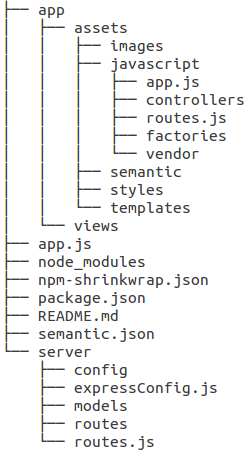
\includegraphics[width=0.5\textwidth]{figuras/directorios.png}
    \caption{Estructura de directorios}
    \label{fig:directorios}
\end{figure}	

\section{Diagramas}
Para una mayor comprensión de la composición del sistema, se han desarrollado diferentes tipos de diagramas.


En la figura \ref{fig:mvc_mvvm_sist} se muestra cómo interactúa el sistema a grandes rasgos a través del patrón MVC-MVVM. No se trata de un diagrama de clases, pero sirve para tener visión general de los distintos elementos que componen el sistema. En amarillo, aparecen elementos de Angular utilizados y se podrían interpretar como los patrones (en azul) que se indican a su lado.


\begin{figure}[htbp] 
    \centering
    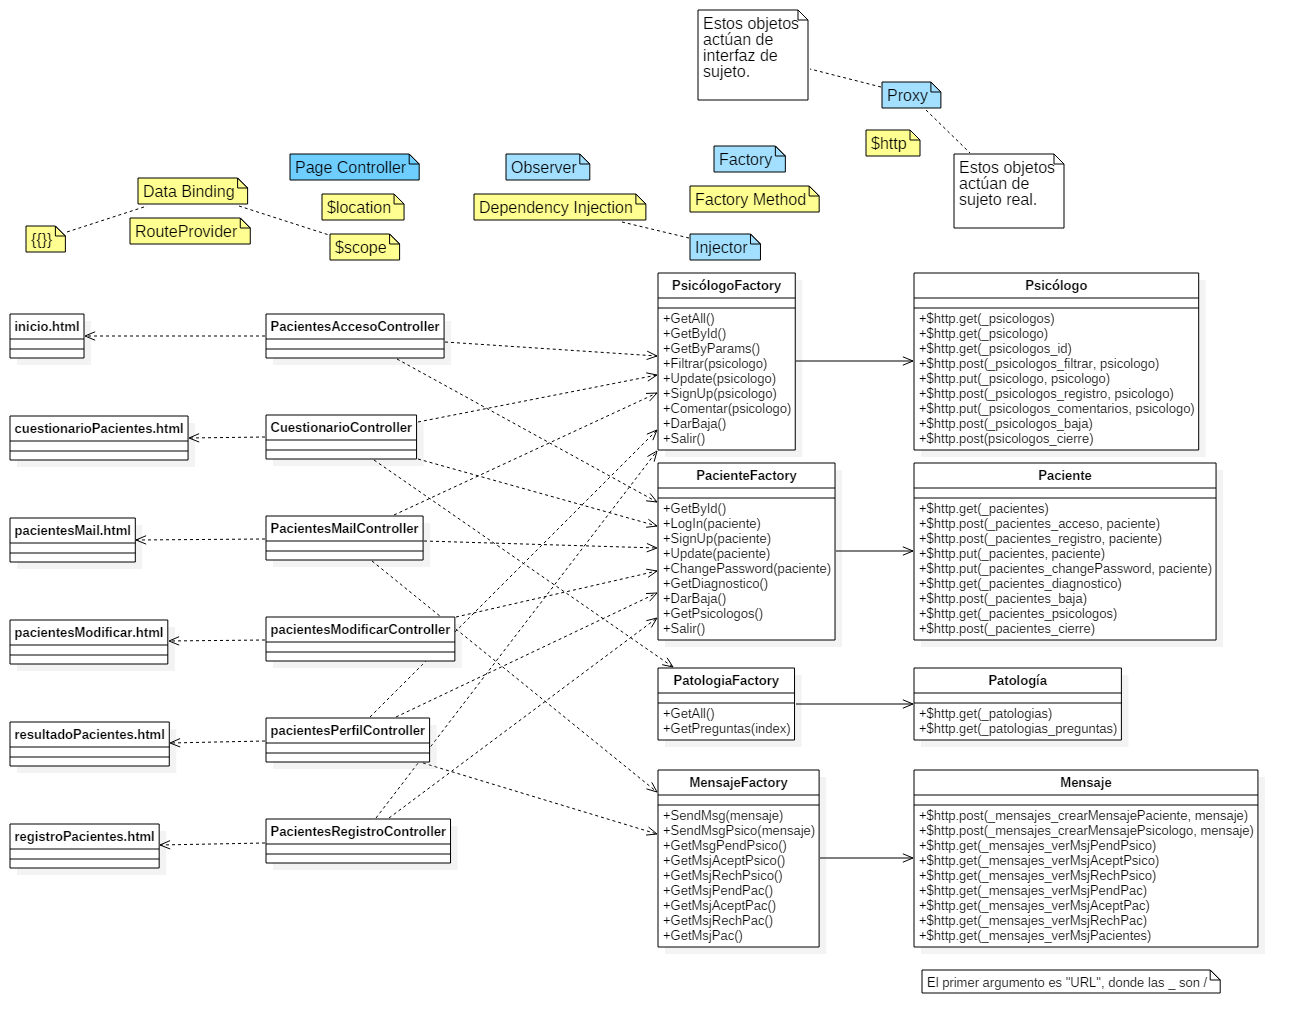
\includegraphics[width=1\textwidth]{figuras/diagrama/MVC.png}
    \caption{Patrón MVC-MVVM}
    \label{fig:mvc_mvvm_sist}
\end{figure}	


En la figura \ref{fig:data_mapper}, se muestra cómo se implementa la capa de datos \textit{Data mapper} con ayuda de los \textit{schemas} y funciones propias de la librería \textit{Moongoose}.


\begin{figure}[htbp] 
    \centering
    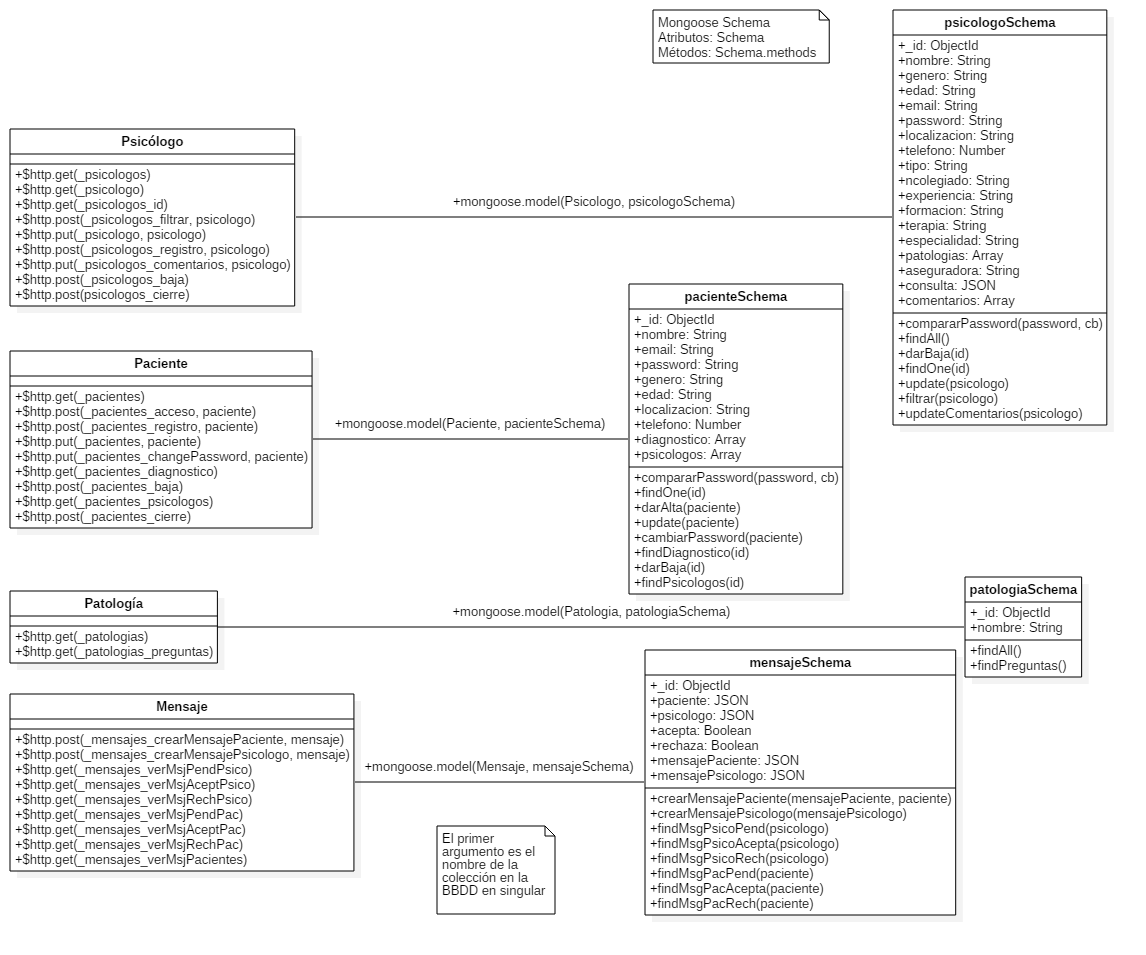
\includegraphics[width=1\textwidth]{figuras/diagrama/Schema_data_mapper.png}
    \caption{Data mapper}
    \label{fig:data_mapper}
\end{figure}	


Para ejemplificar las interacciones entre los distintos componentes del sistema, se han creado dos diagramas de secuencia: Uno referente al caso de uso CU-003 Realizar cuestionario\ref{fig:diag_sec_cu003} y otro del CU-005 Contactar psicólogo\ref{fig:diag_sec_cu005}.


\begin{landscape}

\begin{figure}[htbp] 
    \centering
    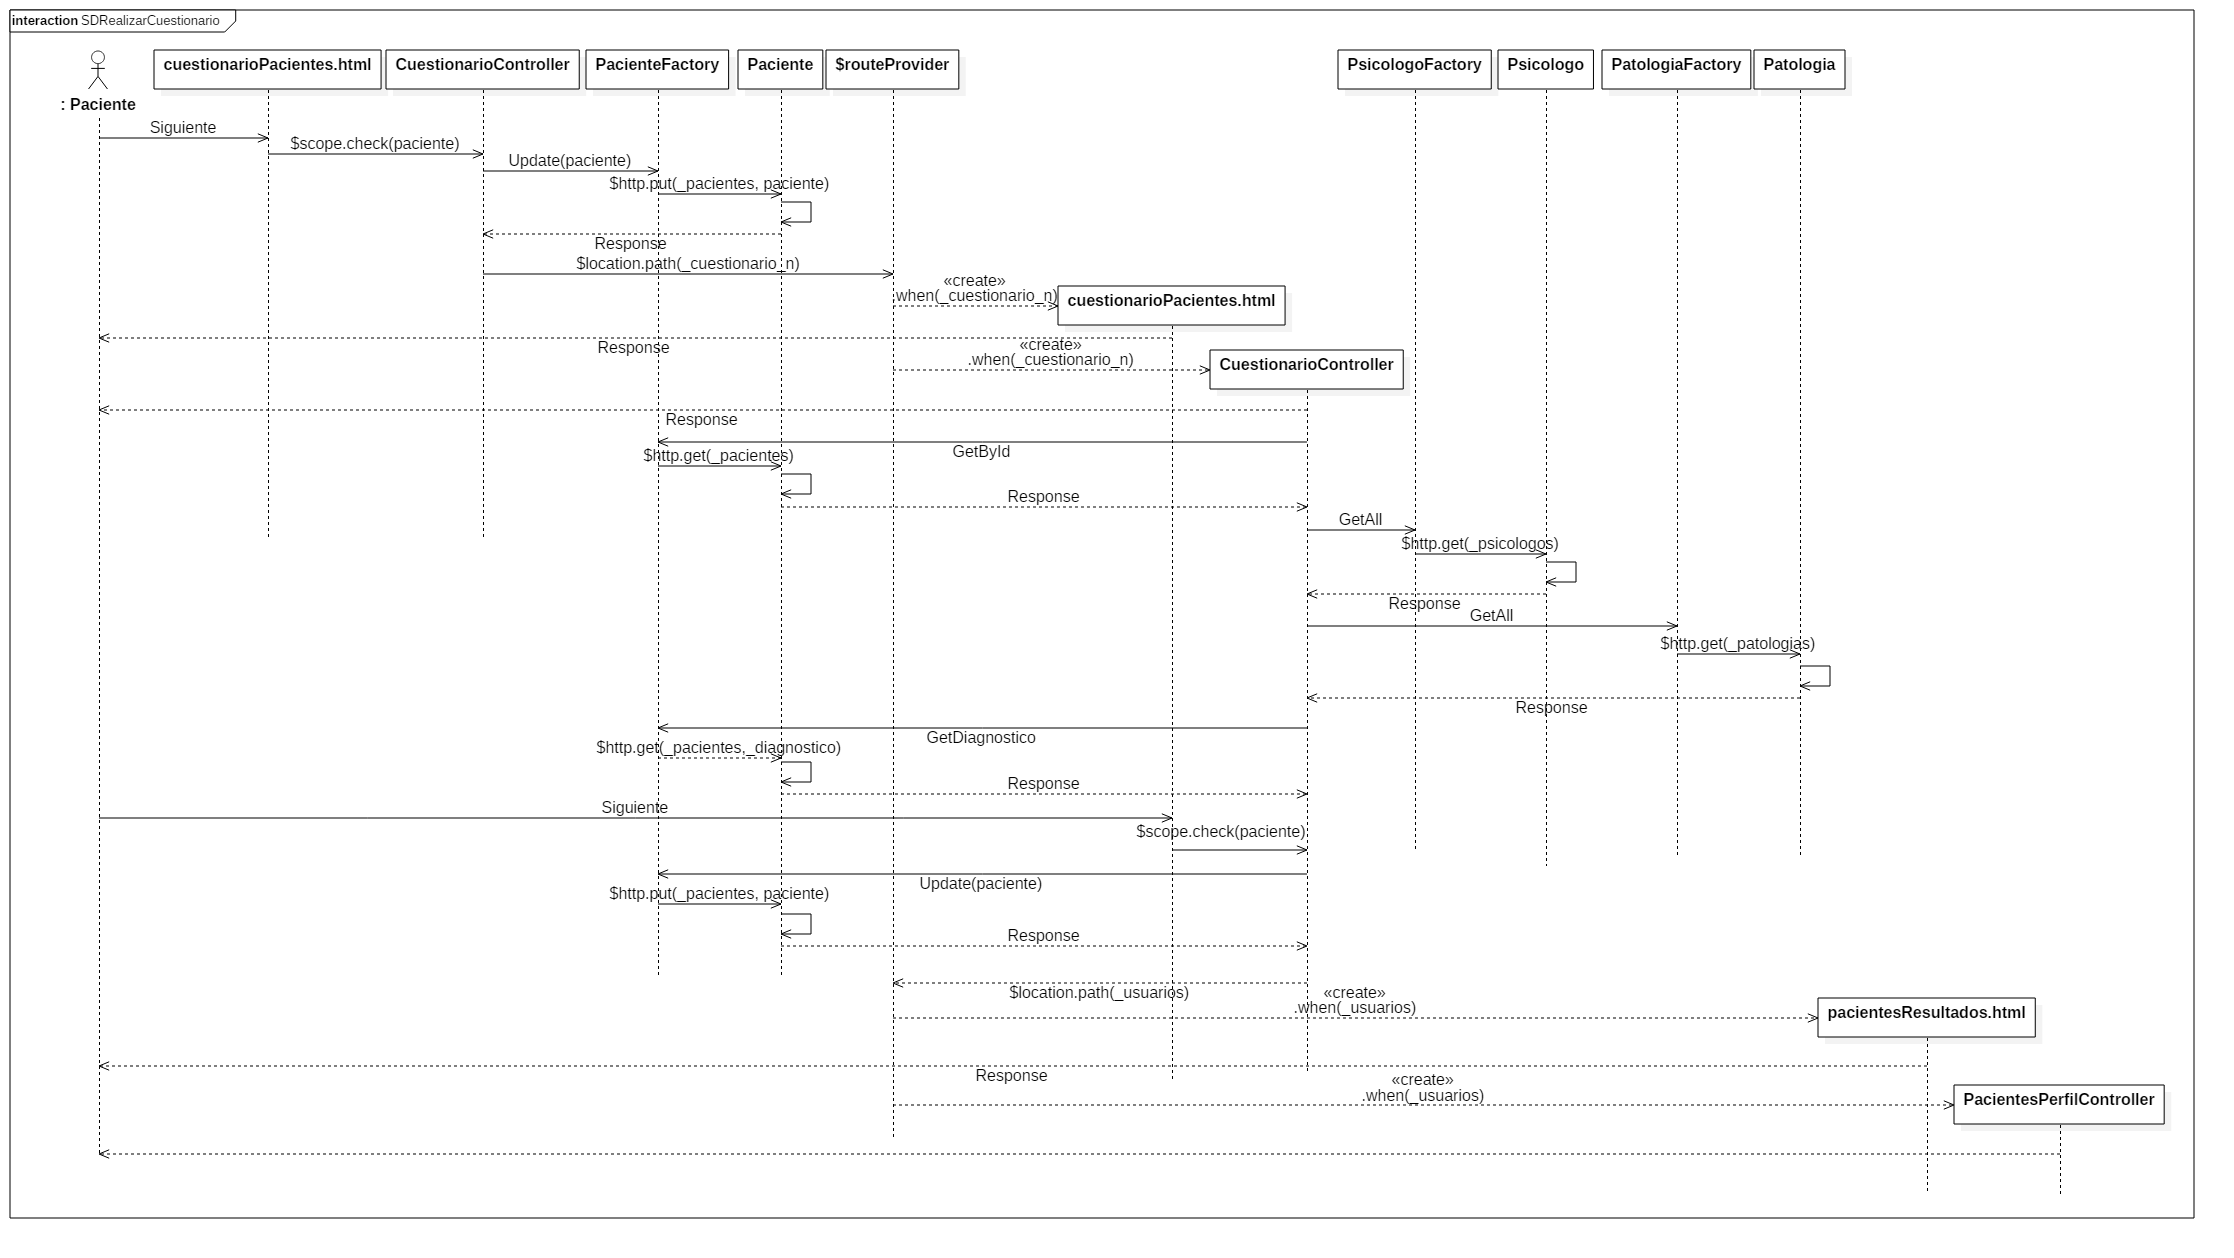
\includegraphics[height=0.8\textwidth,keepaspectratio]{figuras/diagrama/SDRealizarCuestionario.png}
    \caption{Diagrama de secuencia del CU-003}
    \label{fig:diag_sec_cu003}
\end{figure}	

\end{landscape}


\begin{figure}[htbp] 
    \centering
    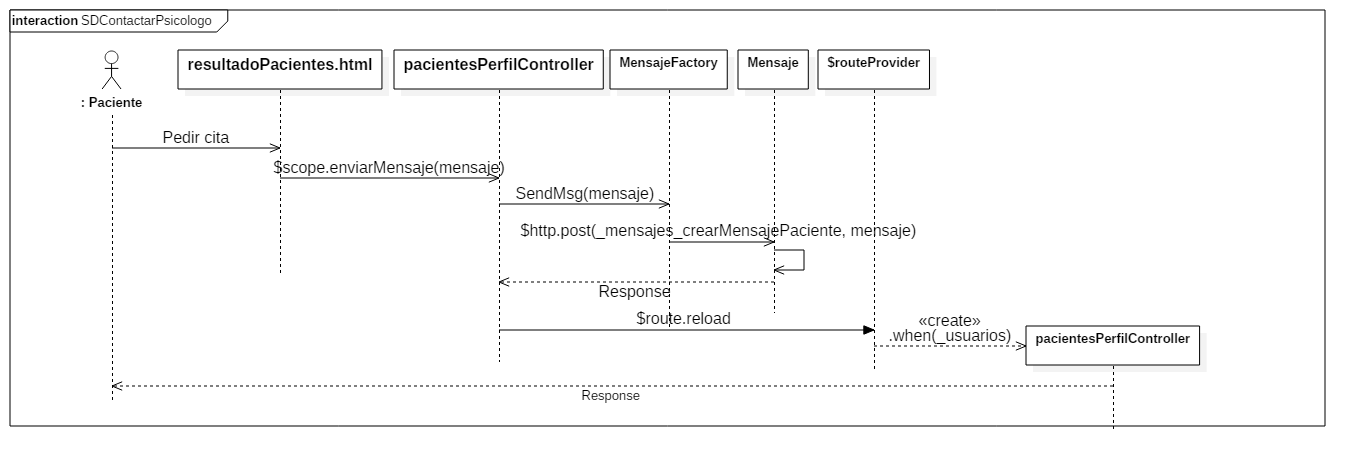
\includegraphics[width=1\textwidth]{figuras/diagrama/SDContactarPsicologo.png}
    \caption{Diagrama de secuencia del CU-005}
    \label{fig:diag_sec_cu005}
\end{figure}	